\chapter{Evaluation}
\label{sec:evaluation}

% Zu jeder Arbeit in unserem Bereich gehört eine Leistungsbewertung. Aus
% diesem Kapitel sollte hervorgehen, welche Methoden angewandt worden,
% die Leistungsfähigkeit zu bewerten und welche Ergabnisse dabei erzielt
% wurden. Wichtig ist es, dem Leser nicht nur ein paar Zahlen
% hinzustellen, sondern auch eine Diskussion der Ergebnisse
% vorzunehmen. Es wird empfohlen zunächst die eigenen Erwartungen
% bezüglich der Ergebnisse zu erläutern und anschließend eventuell
% festgestellte Abweichungen zu erklären.

\ldots evaluation \ldots

\todo{Write evaluation}

\section{Qualitative Analysis}


\begin{table}[H]
    \tiny
    \caption{Possible Vulnerability in upstream Quark in the context of Confidential Computing and suggested Solutions}
    \label{crouch}
    \begin{tabular}{  p{3.4cm}  p{3.4cm}  p{3.4cm} p{2cm} }
        \toprule
\textbf{Vulnerability}      
& \textbf{Attack Example}   
& \textbf{Possible Solution}
& \textbf{Comment}  \\\midrule
Physical Access Attacks
& Offline DRAM Analysis          
& Running the application in a secure virtual machine
& Out of the scope   \\\hline
Lack of protection to guest memory and register states          
& Hypervisor reads private guest memory/cpu states                          
& Running the application in a secure virtual machine
& Out of the scope   \\\hline
Paravirtualized filesystem sharing mechanism       
& Hypervisor/Untrusted host process reads application’s credentials stored on host
& Enable file system shielding layer to encrypt outbound and decrypt inbound data 
& Out of the scope   \\\hline

No security guarantee for communications over the Internet (unbounded network access to containers)     
& Attacker access application’s credential by establishing a network connection to application using tools like, kubectl port-forward
& Enable network shielding layer using TLS
& Out of the scope   \\\hline

Deploying Secrets via untrusted Entities (Kubelet, Containerd, Qvisor)    
& File type secrets are mounted to container rootfs by qvisor, args and envv type secrets are passed to qkernel through qvisor
& Offload the secrets deployment from qvisor by defining a new secure channel btw. relying party and guest kernel for secrets provisioning and storing secrets on guest memory
& Problem solved  \\\hline

Executing arbitrary command in container  
& Attacker view application’s credentials stored on guest memory using kubectl exec cat command
& Enable authentication and access control to kubectl exec in guest kernel
& Problem solved  \\\hline


Container log in plaintext managed by untrusted entity
& Attacker reads application’s log message using kubectl logs container-name
& Enable container STDOUT protection
& Problem solved  \\\hline

Storing Qkernel Log on host in plaintext
& Cloud provider reads guest kernel’s log messages located in directory /var/log/quark
& Enable qkernel log manager and set the log level to OFF
& Problem solved  \\\hline

Loading untrusted executable from host
& Attackers may tamper with executables stored on the host and trick applications into executing compromised code to reveal secrets
& Executable loaded into guest memory is measured and the results are send to relying party for executable integrity check
& Problem solved  \\\hline

Loading untrusted shared library from host
& Attackers may tamper with shared libraries stored on the host and trick applications into executing compromised code to reveal secrets
& Executable loaded into guest memory is measured and the results are send to relying party for executable integrity check
& Problem solved  \\\hline

Missing administration to application restart
& Attacker may provide the guest with compromised executables, shared libraries, or wrong process spec when k8s requests the Qkernel to restart the crashed application
& Compare the hash of the application rebuilding process with the hash of application's initial launching process stored on guest memory. If two hashes doesn’t match,  qkernel refuse the application restart request.
& Problem solved  \\\hline


No restriction to Container's syscalls (guest system calls)
& Applications can be tricked into using vulnerable guest/host system calls, leading to disclosure of secrets
& Using Guest system call interceptor to restrict the system calls application can use.
& Problem solved  \\\hline


Creating application process using untrusted process spec sent from host
& Attacker may trick the qkernel into attaching a terminal to application process by modifying the "terminal" option in the process specification
& Software measurement manager measure the loaded process specification and the results are send to relying party for integrity check
& Problem solved  \\\hline


Lack of runtime measurements
& Secure VM like AMD SEV only calculate the hash of VM launching process, anything loaded to guest during runtime is not measured
& Add software measurement manager to measure data loaded during runtime
& Problem solved  \\\hline
% objects and systems &
% Underlying values       
% & Plurality \\
        \bottomrule
    \end{tabular}
\end{table}


\section{Quantitative Analysis}
In this section, we evaluate the performance of the system implementations described in the previous chapters through multiple benchmarks to assess the impact on the performance and latency of the applications running in the cquark environment.


\subsection{Overview of Quantitative Analysis}


Our benchmarks  consist of micro-benchmarks and macro-benchmarks. The microbenchmarks are performed to  thoroughly understand the latency overhead of each new building block in CQuark, while the macro benchmarks are conducted to compare the speed of 
real world applications run by CQuark vs unmodified Quark, and to get a view of the additional overhead incurred by cquark for protecting application’s confidentiality.


The benchmarking in this section is structured around the following subsections. First, we describe the hardware and software setup for benchmarking in Section 5.1. We then evaluate the speed of obtaining three different types of attestation reports (emulated hardware reports, software reports signed by the kbs key or by the application key) using a microbenchmark that executes a certain number of a system call in a loop and records the time required to execute the system call (Section 2.3). We found that the speed of obtaining the emulated hardware report is 50\% slow than that of obtaining the other two reports due to VM exit. 

Subsequently, in Section 2.4, we evaluate the overhead of the guest system call interceptor using a micro test that executes a certain number of a specific system call in a loop in upstream quark and cquark, respectively. The results show that the guest system interceptor imposes an overhead of 1.47x and 17x for system calls that are handled only by the guest and system calls that must be handled by the host, respectively

Unlike upstream quark, which stores file-type secrets in the host, cquark stores file-type secrets directly on guest memory. Therefore, in Section 2.5, we evaluate the speeds of a application accessing file-type secrets in upstream quark and cquark using a similar approach as in Section 2.4. The results reveal that in cquark, the speed of accessing file-type secrets is improved by a factor of 1.17.


Later, in Section 2.6, we present latency performance benchmark results for sending commands to containers in cquark and upstream quark. Compared to the speed of sending commands using kubectl exec in upstream quark, the authentication and access control for the exec endpoint in cquark introduces 1.15 times overhead. Furthermore, We compare the speed of sending the same command with kubectl and securectl in cquark. The results show that despite the additional encryption and decryption required by the commands sent by securectl, the commands are executed 1.1 times faster than those sent by kubectl.


In Section 2.7, we conducted an evaluation of the latency overhead introduced by the new cquark components during application deployment using a "hello world" program.  Specifically, the evaluation involved testing the latency overhead of the https kbs client, secret injector, shared library measurement manager, hardware evidence driver, and software measurement manager Throughout the experiments, we adjusted a critical parameter to observe how each component affects the overall application startup time Findings indicate that the https kbs client constitutes the bulk of the overhead when the size of the measurement data is less than 100 MB, while the overhead introduced by the secret injector and hardware evidence driver is negligible in any case. Further details, including the benchmark configuration and results can be found on page XX.


In Section 2.8, we conclude the performance benchmarking exercise by conducting macro benchmarking using nginx and redis as workloads. Our benchmarks focus on exploring the performance differences between applications running in cquark and upstream quark in terms of startup time, exit time, and the speed of processing requests during runtime. Our findings reveal that in cquark, redis and nginx require 1.49X and 1.55X startup times than in upstream quark, respectively. The difference primarily arises from the contrast in data size measured during application startup, i.e., 67.15 Mib in Nginx and 16.258 MiB in Redis. In terms of application exit time, Redis and Nginx exhibit nearly identical performance when running on cquark and upstream quark. Furthermore, we utilized Redis-benchmark and Apache HTTP server benchmarking tool as load generators to gauge the application runtime performance. Our experiment results indicate that Nginx and Redis running in cquark encounter performance declines of approximately 9\% and 20\%,respectively,due to guest system interceptor.

\subsection{Hardware and Software Setup}

In this section, a summary of the hardware and software settings utilized for the benchmarks is provided. Regarding hardware, all measurements were performed on an a server with AMD EPYC 7443P 24-Core cpu and 4 DDR4-3200 Mhz-16GB RAM. In terms of software, the host OS is Ubuntu 20.04.6 LTS and Linux 5.19.0 kernel. . To establish a low-noise environment for benchmarking with reproducible results and low variability, the CPU governor was set to performance mode, and Hyper-Threading and Turbo Boost were disabled.  Moreover, all binaries used for testing, i.e. Qvisor, Qkernel, and All binaries used for testing, namely Qvisor, Qkernel, and the "hello-world" application, were built in release mode. Note that, unless otherwise mentioned, the unchanged version of Quark, i.e., upstream Quark is v0.2.0 in the following.


Regarding the tools for measuring latency, since all benchmark objects are located in the guest, we use the guest system call clock\_gettime(monotonic) for time measurement and print the results to the host using the qkernel logging system. The benchmarking framework can analyze the benchmarking results by parsing the cquark log located under host directory /var/log/quark.

In addition, all benchmark tests are performed multiple times to minimize the impact of environmental noise on the data results. Figures in the following sections illustrate the measurement results, conveying the average time and variance utilized for one run of the subject being measured.


\subsection{Micro-benchmark – Attestation Report Syscall}

Cquark enables guest user mode applications to obtain three types of attestation reports, that is, simulated AMD SEV SNP reports, software reports signed by KBS keys, or software reports signed by the application via a system call. In this section, we assess the speed with which the application 
acquires various attestation reports.

\begin{figure}[H]
    \centering
    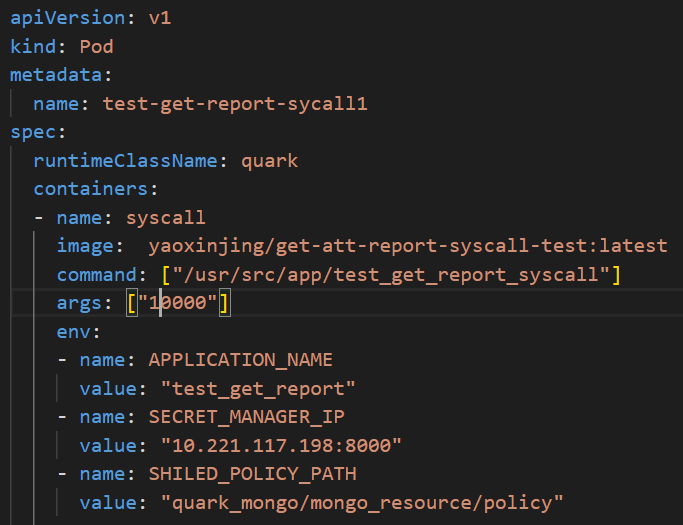
\includegraphics[width=0.8\textwidth]{images/perf_attestation_report_yaml.PNG}
    \caption[Qkernel Attestation Report Syscall Benchmark Deployment]{Qkernel Attestation Report Syscall Benchmark Deployment}
    \label{fig:perf_attestation_report_yaml}
\end{figure}

To this end, we prepared a Rust microbenchmark that measures the mean and variance of the time requisite for obtaining the three types of reports and prints the results to its standard output. To ensure stable outcomes, the test program submits 10,000 requests for each type of report to the kernel. 
As the benchmark program is containerized, we can deploy the benchmark to Cquark using the YAML file in Figure ~\ref*{fig:perf_attestation_report_yaml}.

\begin{figure}[H]
    \centering
    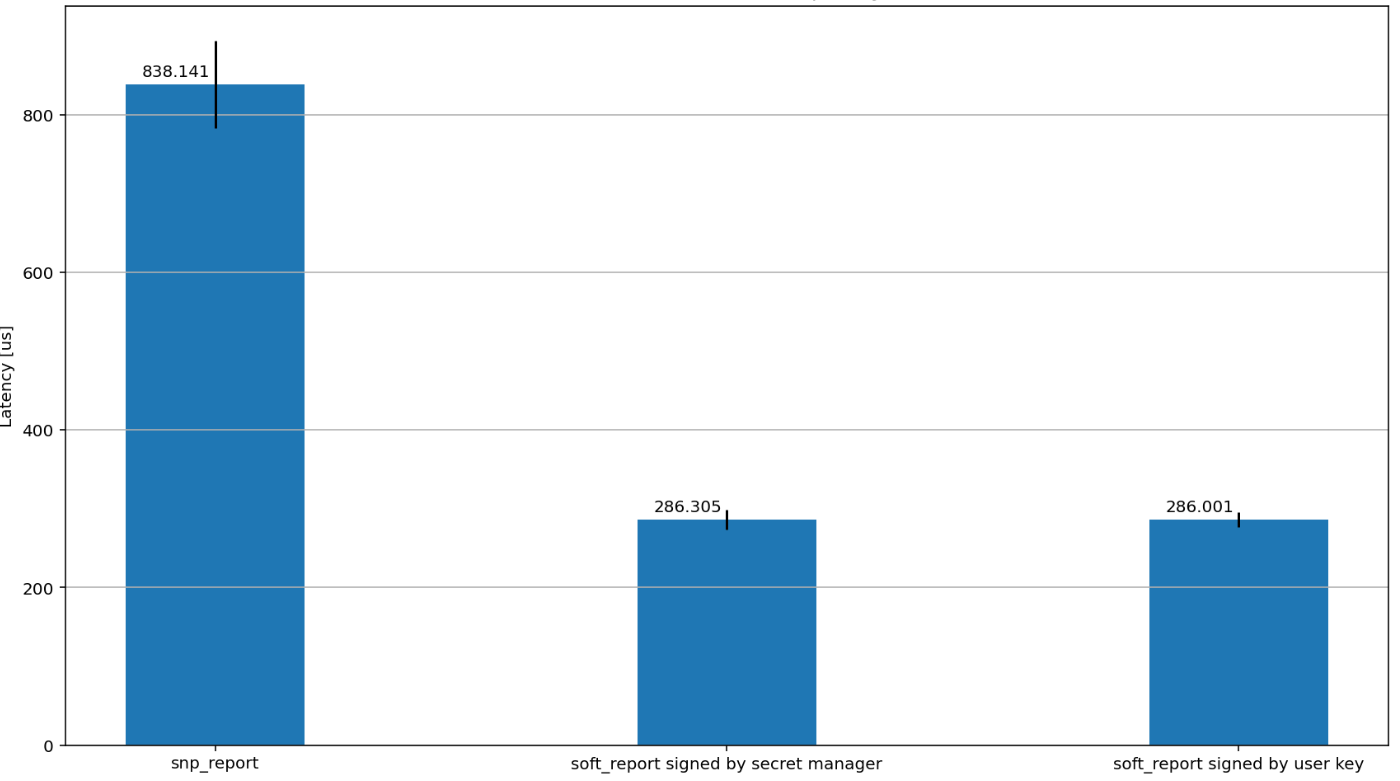
\includegraphics[width=0.8\textwidth]{images/perf_attestation_report_result.PNG}
    \caption[Benchmark result of Attestation Report Syscall]{Qkernel Attestation Report Syscall Benchmark Deployment}
    \label{fig:perf_attestation_report_result}
\end{figure}

Figure \ref{fig:perf_attestation_report_result} depicts the speed of requesting three types of proof reports for guest mode applications in the cquark setting. The data reveal that acquiring a software report requires approximately one-third of the time needed to obtain a simulated hardware report. 
Specifically, requesting a simulated hardware report takes approximately 838.141us, whereas acquiring the two software reports needs only about 286us. The disparity stems from the dissimilarities in processing software and hardware reports by the qkernel. While the qkernel 
system call handler generates software reports promptly, the handler needs to transmits hardware report requests through qkernel snp attestation driver to the host AMD SEV emulation module in order to generate a dummy report. This process involves a lot expensive operations like VM exit, 
encryption and decryption of messages for communication between the snp attestation driver and host AMD SEV emulation modul, reading the on-disk dummy snp report among others. Consequently, acquiring a simulated hardware repors is significantly slower than obtaining a software report.


\subsection{Micro-benchmark – Qkernel Syscall Interceptor}

Interception of guest system calls by the guest system call interceptor to determine whether a call is legitimate introduces latency overhead to applications running in the guest user mode.  To investigate this overhead, we employ a micro benchmark program written in Rust.  The benchmark measures the average and variance execution time of chosen system calls. Furthermore, to obtain stable results., each system call is executed in a loop of 100,000 times. As the benchmark program is containerized, we can deploy the program to Cquark and upstream Quark using the YAML file in Figure \ref{fig:syscall_interceptor_yaml}.
\begin{figure}[H]
    \centering
    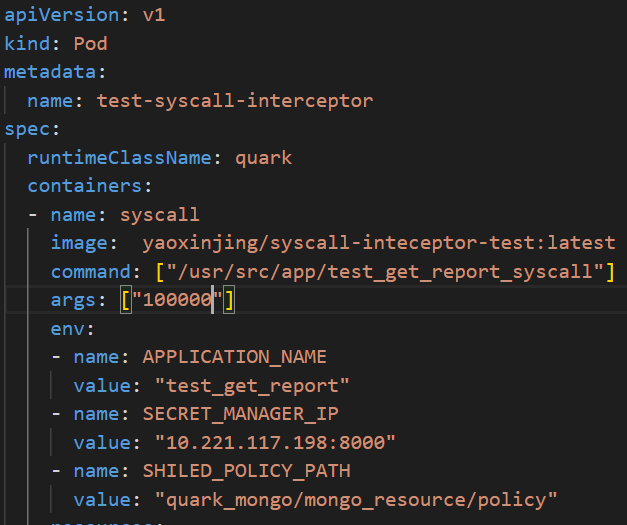
\includegraphics[width=0.8\textwidth]{images/perf_system_call_interceptor_yaml.PNG}
    \caption[Qkernel Syscall Interceptor Benchmark Deployment]{Qkernel Syscall Interceptor Benchmark Deployment}
    \label{fig:syscall_interceptor_yaml}
\end{figure}


For this benchmark, we select four system calls: getpid, getppid, read, and write. Since qkernel already implements process and thread objects, calling getpid or getppid prompts qkernel to directly return the corresponding pid/ppid without interference from the host. This provides us with a clear understanding of the overhead introduced by the interceptor. Additionally, we measured the execution time of read and write system calls for Cquark and upstream Quark to evaluate the overhead that the interceptor brought to the host-handled system calls
\begin{figure}[H]
    \centering
    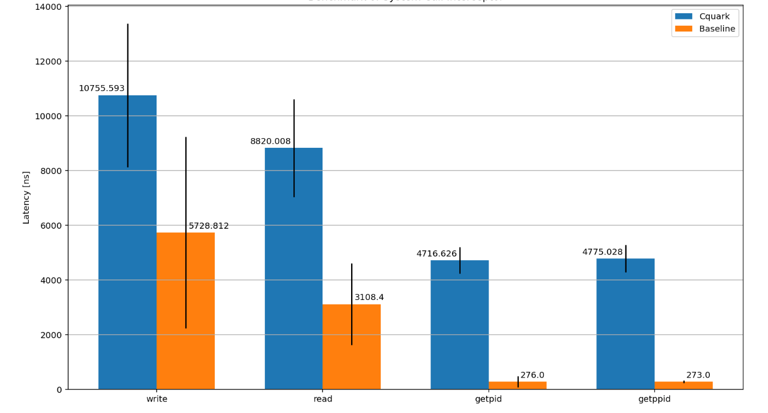
\includegraphics[width=0.8\textwidth]{images/ben_results_syscall_interceptor.PNG}
    \caption[Benchmark result of Syscall Interceptor]{Latency comparison of executing syctem calls in Cquark vs upstream Qaurk. The latency is thereby measured using the guest system call clock\_gettime(monotonic). 
        Each system call is executed 1,000,000 times in a tight loop. Read and write buffer size is 100 bytes}
    \label{fig:ben_results_syscall_interceptor}
\end{figure}


Figure ~\ref{fig:ben_results_syscall_interceptor} illustrates the mean and variance of execution times for the selected system calls in the upstream Quark and Cquark environments. We observed that upstream Quark takes only around 270 ns to execute a single getpid and getppid call while Cquark takes approximately 4716 ns. This implies that the guest system call interceptor causes a delay of about 4500 ns per system call. Moreover, a comparable latency overhead is introduced for read and write system calls, i.e.,4500 ns.  However, since read and write system calls are processed on the host side and take longer, their processing time in Cquark does not rise as significantly as that of getpid and getppid. To summarize, in cquark, host handled system calls in the (i.e., write and read) and guest handled-only (e.g., getpid and getppid) are 1.47x and 17x slower, respectively, compared to upstream Quark


The overhead incurred by the system call interceptor arises from two primary sources. Firstly, the whitelist of client-side system call interceptors is kept in a vector. Accessing the whitelist for system call authorization check is an operation with the complexity of O(N). Secondly, to avert any contentions resulting from run-time updates and reads to the system call interceptor's metadata, this metadata is safeguarded with a lock. Consequently, a lock/unlock operation is initiated for every system call permission check.



\subsection{Micro-benchmark – Speed of Reading file base secret}

Compared to upstream Quark which stores file type secrets on the host, CQuark instead stores them in guest memory to prevent unauthorized access and avoid potential VM exits during read and write operations. Hence, the purpose of this benchmark is to evaluate the performance enhancement achieved from 
accessing file type secrets in CQuark. The benchmark measures the total time taken to perform one open() and read() operation on a target secret type file in both upstream Quark and CQuark environments. The file size is 1302 bytes. To ensure stable results, 10,000 open and read operations are performed.
As the benchmark program is containerized, we deploy it to both CQuark and upstream Quark using the YAML file outlined in Figure ~\ref{fig:file_type_secret_access_test_deploy_yaml_baseline} and ~\ref{fig:file_type_secret_access_test_deploy_yaml_cquark}.


% \begin{figure}[H]
%     \centering
%     \subfloat[\centering Deployment File for upstream Quark]{{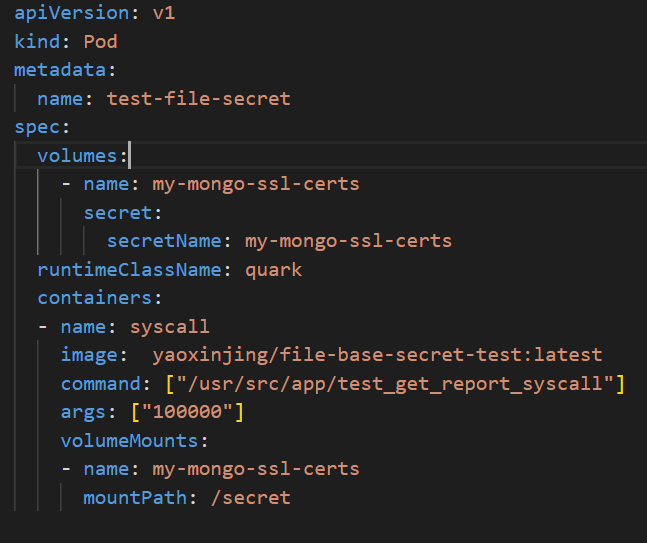
\includegraphics[width=5cm]{images/file_type_secret_access_test_deploy_yaml_baseline.PNG} }}
%     \qquad
%     \subfloat[\centering Deployment File for confidential Quark]{{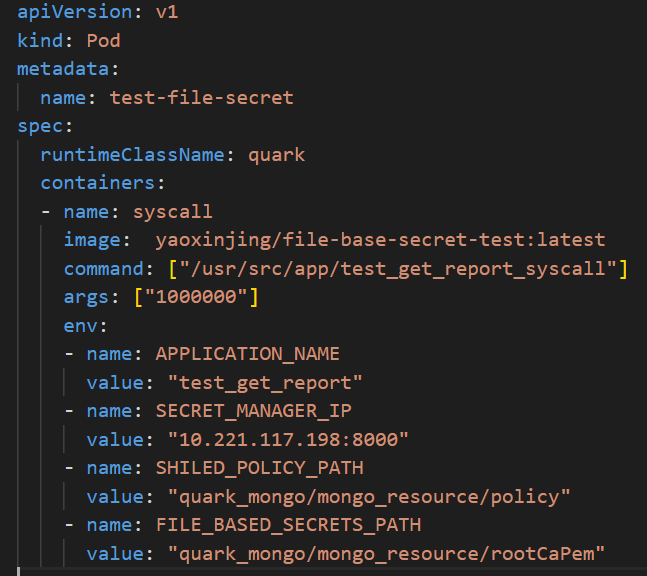
\includegraphics[width=5cm]{images/file_type_secret_access_test_deploy_yaml_cquark.PNG} }}
%     \caption{Benchmark Deployment for testing Speed of Reading file type Secrets }
%     \label{fig:file_type_secret_access_test_deploy_yaml_baseline}
% \end{figure}
% \end{document}

\begin{figure}
    \centering
    \begin{minipage}{0.45\textwidth}
        \centering
        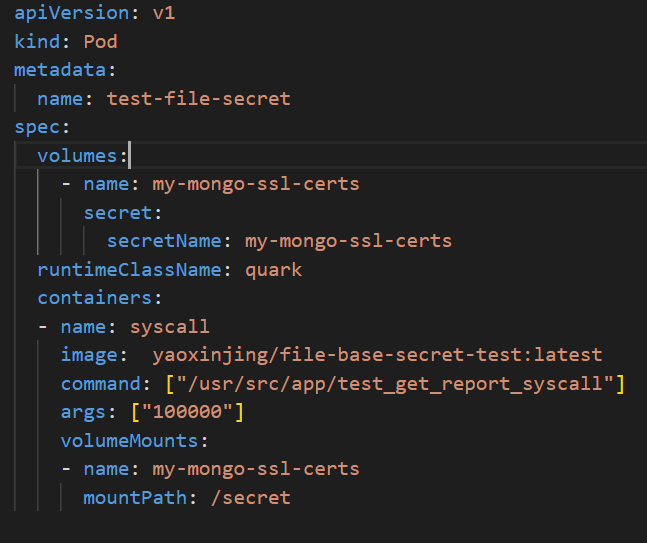
\includegraphics[width=0.9\textwidth]{images/file_type_secret_access_test_deploy_yaml_baseline.PNG} % first figure itself
        \caption{Benchmark Deployment for testing Speed of accessing file type Secrets in upstream Quark}
        \label{fig:file_type_secret_access_test_deploy_yaml_baseline}
    \end{minipage}\hfill
    \begin{minipage}{0.45\textwidth}
        \centering
        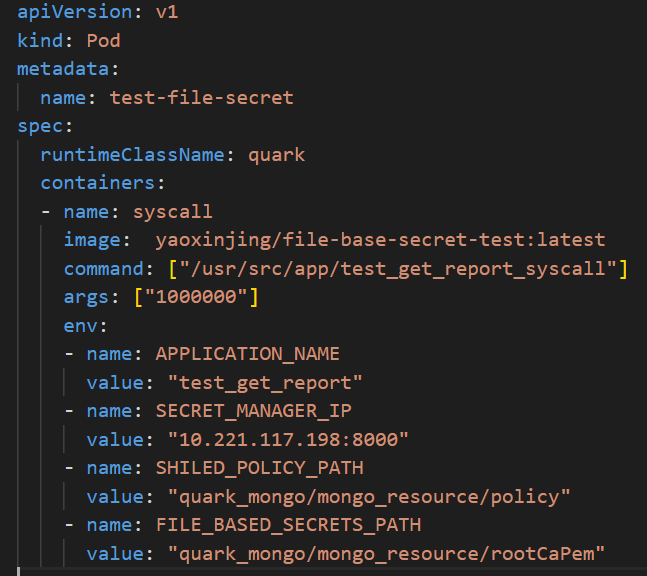
\includegraphics[width=0.9\textwidth]{images/file_type_secret_access_test_deploy_yaml_cquark.PNG} % second figure itself
        \caption{Benchmark Deployment for testing Speed of accessing file type Secrets in confidential Quark}
        \label{fig:file_type_secret_access_test_deploy_yaml_cquark}
    \end{minipage}
\end{figure}


\begin{figure}[H]
    \centering
    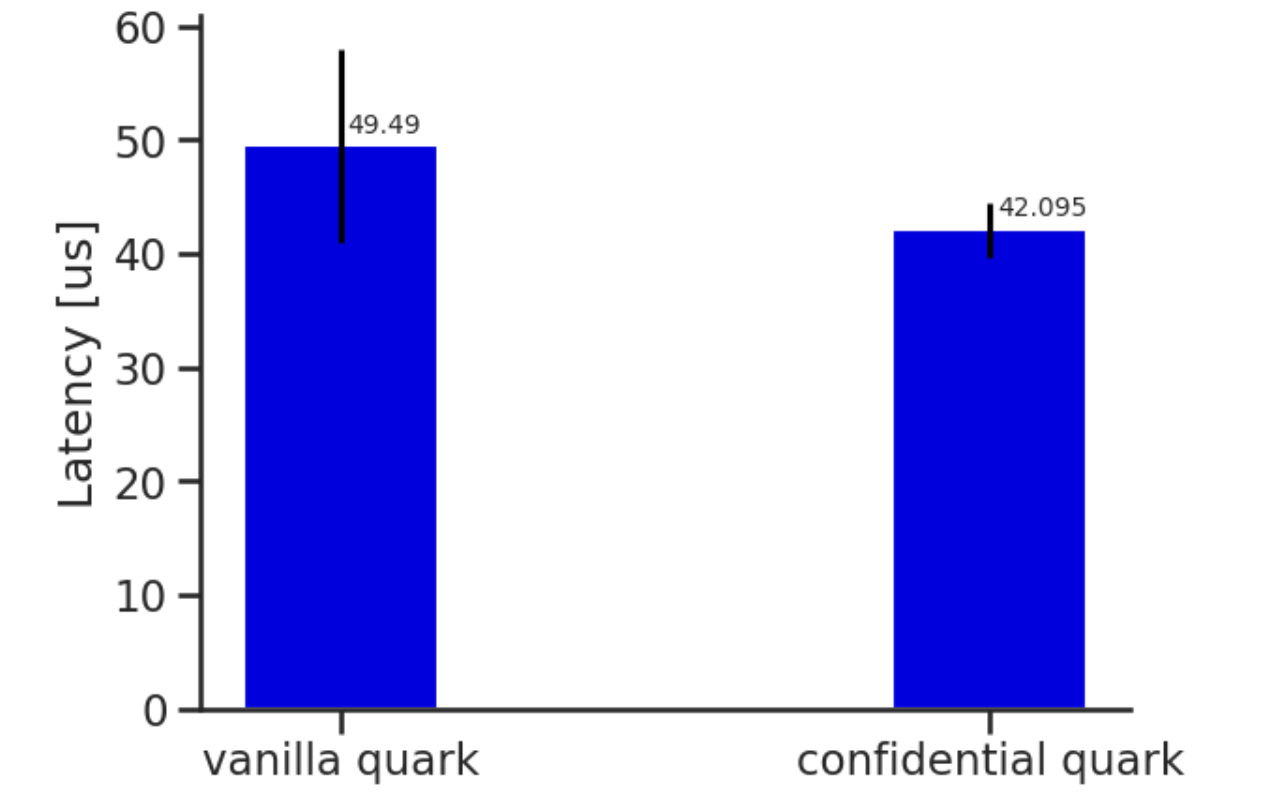
\includegraphics[width=0.8\textwidth]{images/reading_speed_of_file_type_secrets_in_Baseline_and_Cquark.PNG}
    \caption[Benchmark result of testing Speed of accessing file type Secrets in confidential Quark vs upstream quark]{The figure shows result of testing speed of accessing file type secrets in confidential Quark vs upstream Quark. 
    The evaluations is performed using the open() and read() system calls, and ten thousand (10,000) operations are conducted with a 50-byte read buffer size.
    }
    \label{fig:reading_speed_of_file_type_secrets_in_Baseline_and_Cquark}
\end{figure}


The obtained results are presented in Figure ~\ref{fig:reading_speed_of_file_type_secrets_in_Baseline_and_Cquark}, revealing that the performance of s in CQuark is competitive with upstream Quark for accessing file-type secrets. Surprisingly, there is no significant difference in speed between the two, with CQuark providing only 1.17 times the performance improvement when accessing the target secret file.  This reason is that the larger performance loss resulting from system call execution due to the client system call interceptor in CQuark outweighs the overhead produced by VM exits in upstream Quark.


\subsection{Micro-benchmark – Latency Test for issuing Instructions to Application}

This section presents the results of tests conducted to assess the latency of issuing instructions to applications in Cquark. The tests involved comparing the latency of sending commands using kubectl between Cquark and midstream Quark, as well as a speed comparison test for issuing unprivileged 
and privileged commands in Cquark using kubectl and securectl respectively.


To facilitate the tests, we extended our test framework to enable it to issue specific instructions to the application using either kubectl or securectl, while recording command execution time. Similar to previous benchmarks, each instruction was iterated 1,000 times to ensure dependable results. 
Due to time constraints, we were unable to measure all available commands on the Linux system, so we chose four commonly used commands for the following testing: pwd, ls, cat, and cp.

% \begin{figure}
%     \centering
%     \begin{minipage}{0.45\textwidth}
%         \centering
%         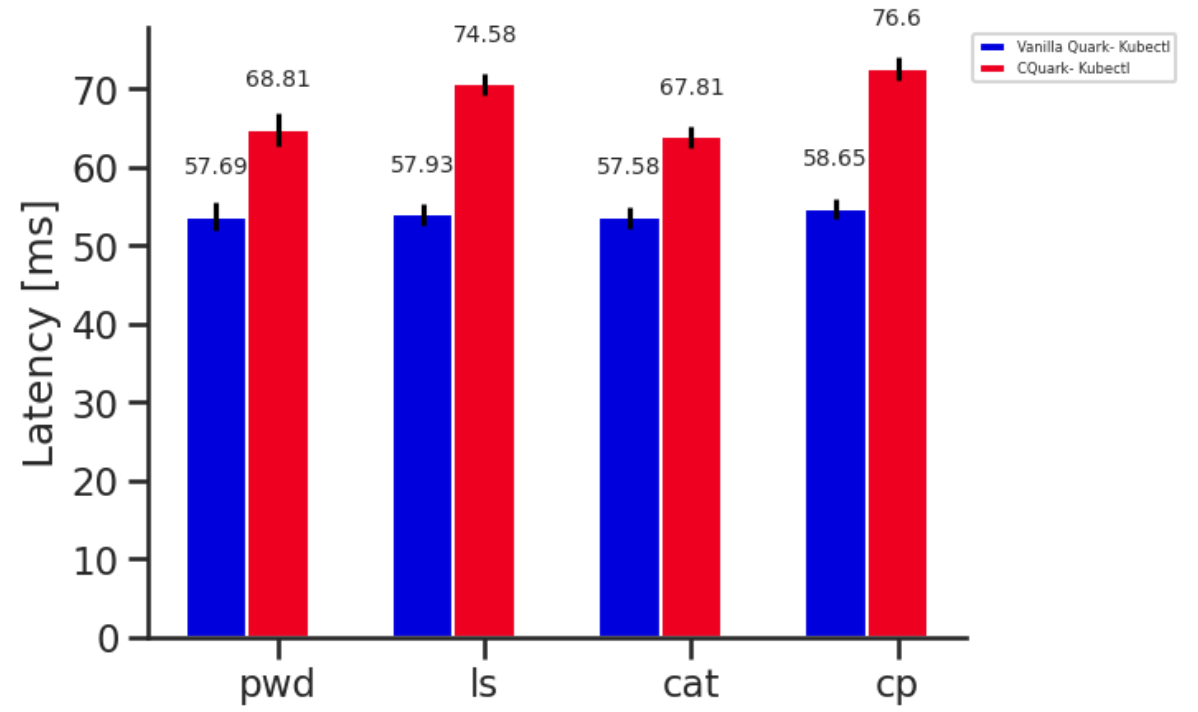
\includegraphics[width=0.9\textwidth]{images/speed_of_issuing_cmd_in_cquark_upstream_quark.PNG} % first figure itself
%         \caption{Benchmark Deployment for testing Speed of accessing file type Secrets in upstream Quark}
%         \label{fig:speed_of_issuing_cmd_in_cquark_upstream_quark}
%     \end{minipage}\hfill
%     \begin{minipage}{0.45\textwidth}
%         \centering
%         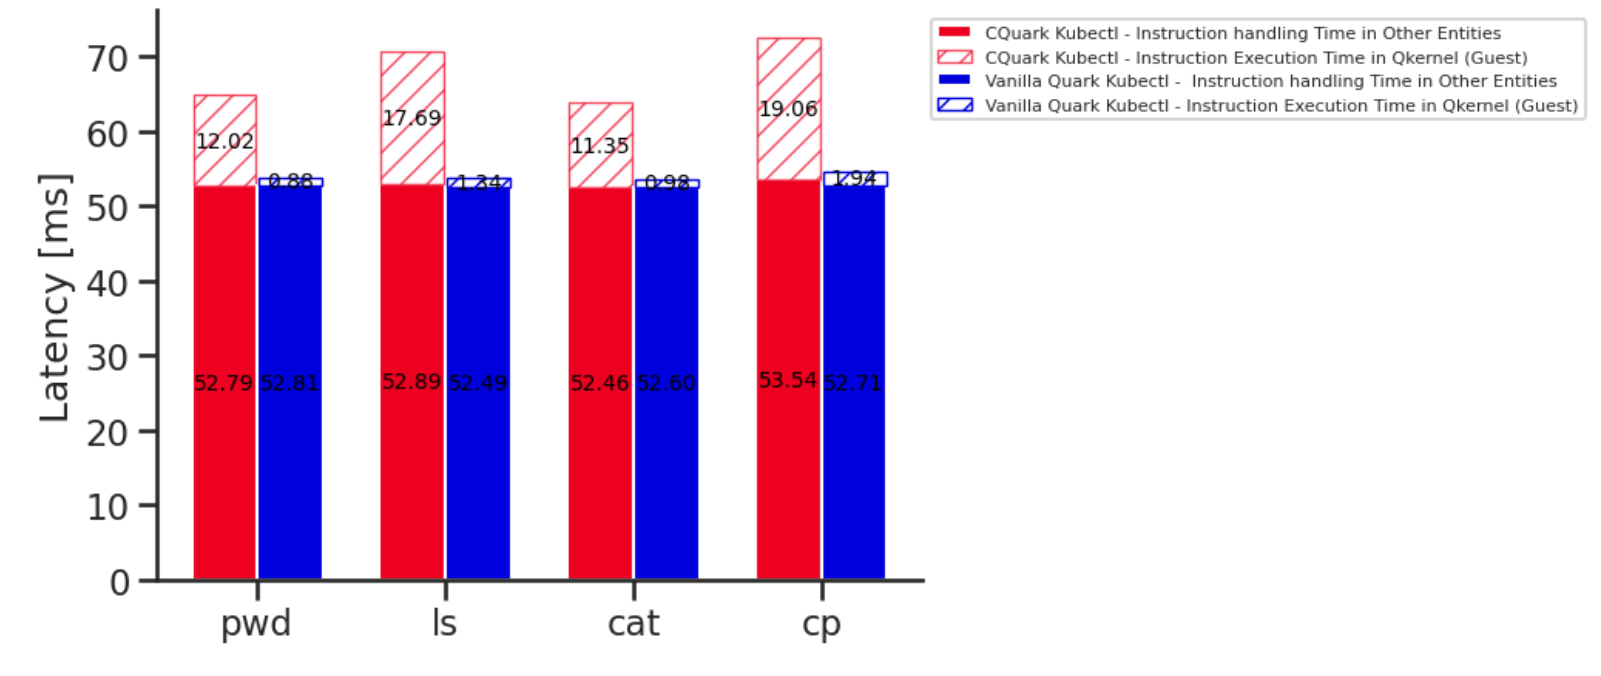
\includegraphics[width=0.9\textwidth]{images/timeshare_issuing_cmd_in_cquark_upstream_quark_kubectl.PNG} % second figure itself
%         \caption{Benchmark Deployment for testing Speed of accessing file type Secrets in confidential Quark}
%         \label{fig:timeshare_issuing_cmd_in_cquark_upstream_quark_kubectl}
%     \end{minipage}
% \end{figure}

\begin{figure}[H]
    \centering
    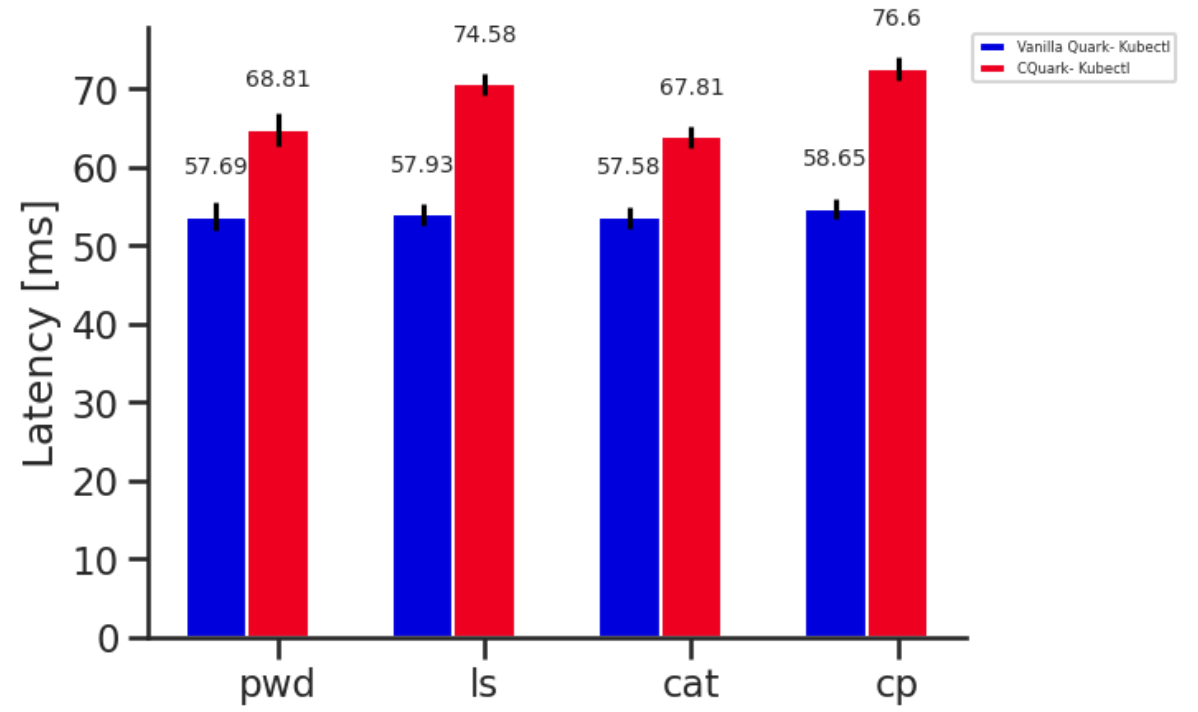
\includegraphics[width=0.8\textwidth]{images/speed_of_issuing_cmd_in_cquark_upstream_quark.PNG}
    \caption[Benchmark result - Latency Comparison of sending Commands to Application in Cquark vs vanilla Quark]{A latency comparison test of sending commands to applications in cquark vs vanilla quark.  The test selects four 
    commonly used Linux commands as samples, each being executed one thousand times. The results indicate that utilizing Kubectl exec to issue instructions to applications in cquark takes over 9\% longer than in vanilla quark.
    }
    \label{fig:speed_of_issuing_cmd_in_cquark_upstream_quark}
\end{figure}




\begin{figure}[H]
    \centering
    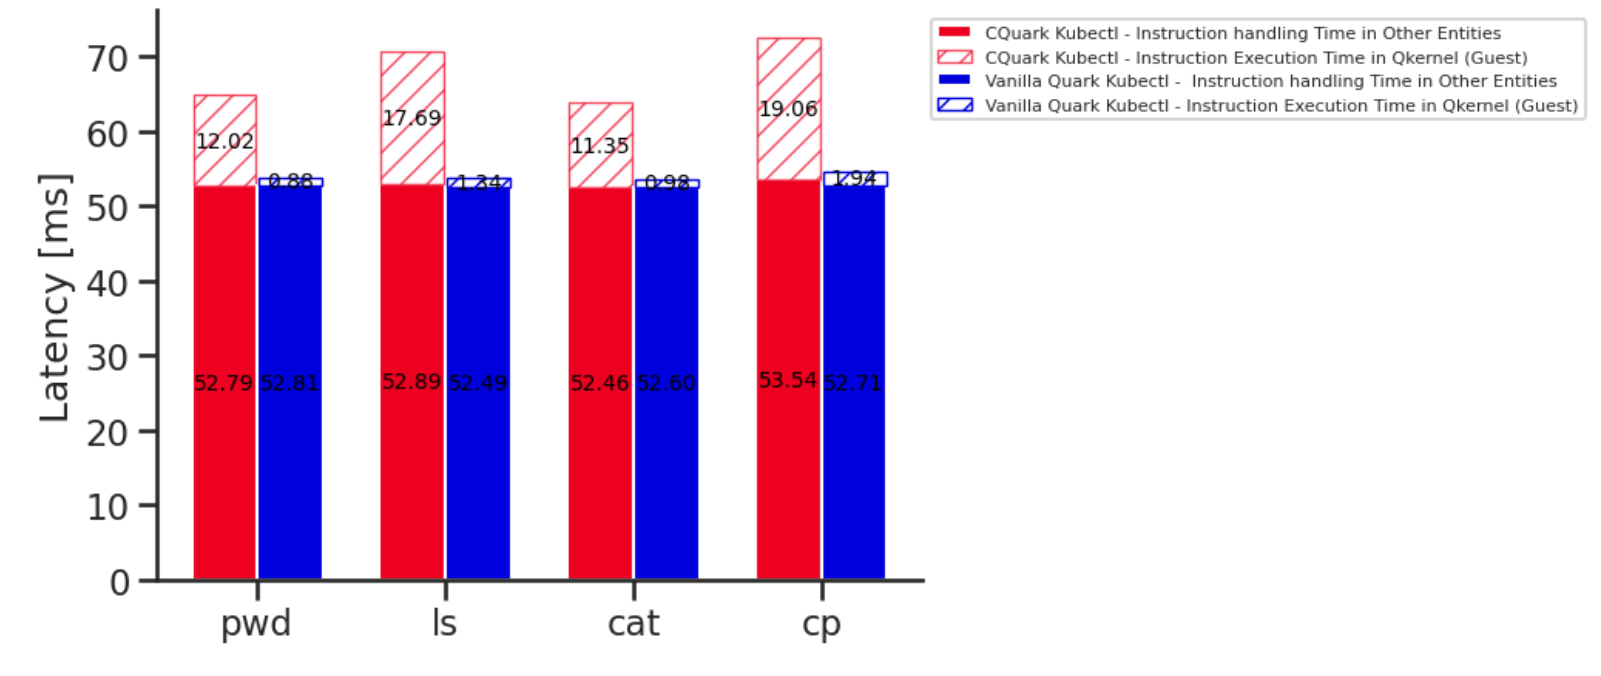
\includegraphics[width=0.8\textwidth]{images/timeshare_issuing_cmd_in_cquark_upstream_quark_kubectl.PNG}
    \caption[Benchmark result - The processing time for each component during the instruction execution lifecycle in Cquark vs in vanilla Quark]{Benchmark result of evaluating the percentage of time spent by each component in processing instructions during the instruction execution lifecycle in Cquark vs in vanilla Quark . Here 
     the components refer kubectl,  Kubernetes components for instructions transmission, like containerd, etc., and Qkernel for instruction execution. 
     Each bar in the figure represents the total execution time of an instruction whereby the color-filled section represents the time qkernel used for instruction execution, while the dashed-filled segment implies the time other components took for instruction issuing, transmission, and result handling.
    }
    \label{fig:timeshare_issuing_cmd_in_cquark_upstream_quark_kubectl}
\end{figure}


This section focuses on analyzing the benchmarking results illustrated in Figures ~\ref{fig:speed_of_issuing_cmd_in_cquark_upstream_quark} and ~\ref{fig:timeshare_issuing_cmd_in_cquark_upstream_quark_kubectl}, which shed light on the overhead generated by the Cquark implementation for issuing instruction to application. The results show that cquark introduces approximately 9\% overhead to the instruction 
execution compared to vanilla quark. This overhead stems from several factors. Firstly, unlike upstream quarks, the Qkernel in Cquark performs authentication and access control in Qkernel for each instruction. Besides, the measurement of the instruction's corresponding binary and guest system call 
interception increases the instruction execution time.  This argument is confirmed in Figure 5.1b, where the average time for Qkernel execution of instructions in a vanilla quark environment is between 1 and 2 ms, while in Cquark, instructions execution in Qkernel takes more than 10 ms. Thus, issuing 
instructions using Kubectl in Cquark proves to be more expensive than in vanilla quark.

\begin{figure}[H]
    \centering
    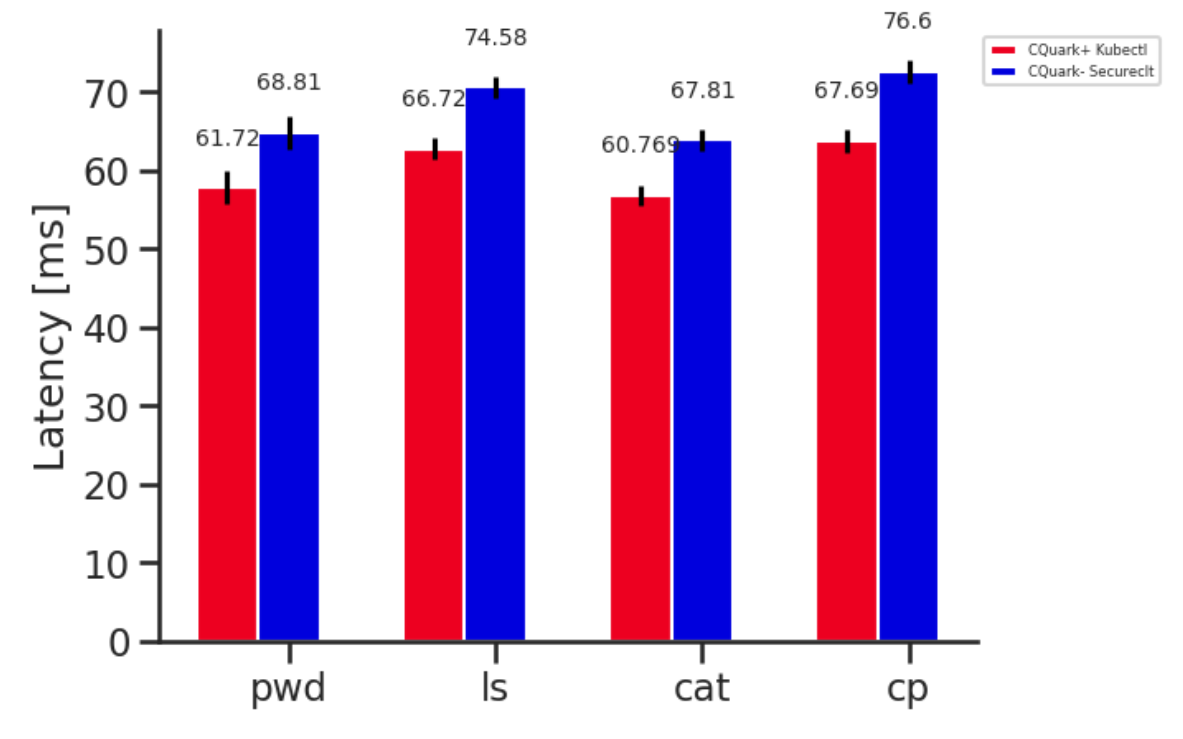
\includegraphics[width=0.8\textwidth]{images/speed_of_issuing_cmd_in_cquark_kubctl_securectl.PNG}
    \caption[Benchmark result - Latency Comparison of issuing privileged instruction vs unprivileged instruction in CQuark]{A latency comparison test of issuing privileged instruction vs unprivileged instruction in CQuark.  The test included four frequently used Linux commands as samples, 
    each being executed one thousand times.The results indicate that issuing privileged instructions is faster than issuing unprivileged instruction.
    }
    \label{fig:speed_of_issuing_cmd_in_cquark_kubctl_securectl}
\end{figure}


Out of curiosity, we compared the time required to issue privileged and unprivileged instructions in Cquark to the application using Securectl and Kubectl, respectively. The results in Figure ~\ref{fig:speed_of_issuing_cmd_in_cquark_kubctl_securectl} reveal that issuing privileged instructions is much faster than issuing unprivileged commands. This finding is counterintuitive since 
privileged instructions require additional cryptographic protection to ensure the confidentiality and integrity of their contents, which implies executing additional code.

\begin{figure}[H]
    \centering
    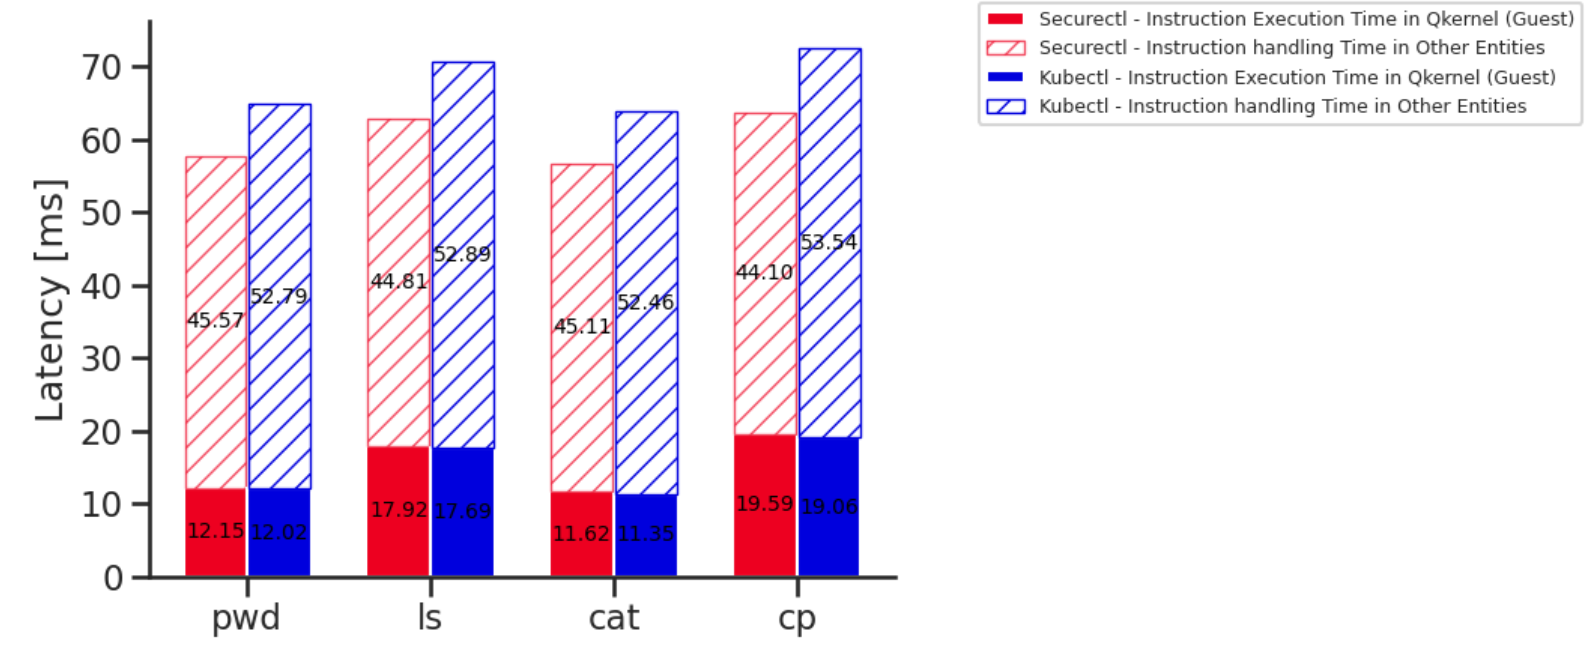
\includegraphics[width=0.8\textwidth]{images/timeshare_issuing_cmd_in_cquark_kubectl_securectl.PNG}
    \caption[Benchmark result - The processing time for components during the privileged vs unprivileged instruction execution lifecycle]{Benchmark result evaluating the percentage of time spent by each component in processing instructions during the privileged versus unprivileged instruction 
    execution lifecycle . Here the components refer to the tool the user employed to issue instructions, i.e., kubectl or securecli,  Kubernetes components for instructions transmission, like containerd, etc., and Qkernel for instruction execution.  Each bar in the 
    figure represents the total execution time of an instruction whereby the color-filled section represents the time qkernel used for instruction execution, while the dashed-filled segment implies the time other components took for instruction issuing, transmission, and result handling.
    }
    \label{fig:timeshare_issuing_cmd_in_cquark_kubectl_securectl}
\end{figure}

To investigate the issue further, we conducted time  measurements of processing time for each component during the privileged vs unprivileged instruction execution lifecycle. Here the components refer to the tool the user employed 
to issue instructions, i.e., kubectl or securecli,  Kubernetes components for instructions transmission, like containerd, etc., and Qkernel for instruction execution.
Figure ~\ref{fig:timeshare_issuing_cmd_in_cquark_kubectl_securectl} presents the results obtained. The time incurred by qkernel for executing unprivileged and privileged instructions (color-filled boxes) distinctly shows that the latter takes approximately 0.5 milliseconds more than the former does. These latency overheads derive from the decryption and 
integrity checks that kernel performs for each privileged instruction, as well as the cryptographic protection for the instruction result. However, comparing the time taken by kubectl and securectl to process user requests (dashed filled boxes), securectl is significantly faster. Thus, this 
offsets the cryptographic protection overhead for privileged instructions.


\subsection{Micro-benchmark – Latency Test for Application Startup}
The introduction of remote attestation, secret provisioning, and data measurement from the host in Cquark results in additional latency overhead for application startup. To examine this overhead, we extended the testing framework to iteratively initiate and terminate the application, measuring the 
start time, exit time, and latency overhead incurred by the remote attestation and provisioning agent, secret injector, hardware evidence driver, and software measurement manager.

\begin{figure}[H]
    \centering
    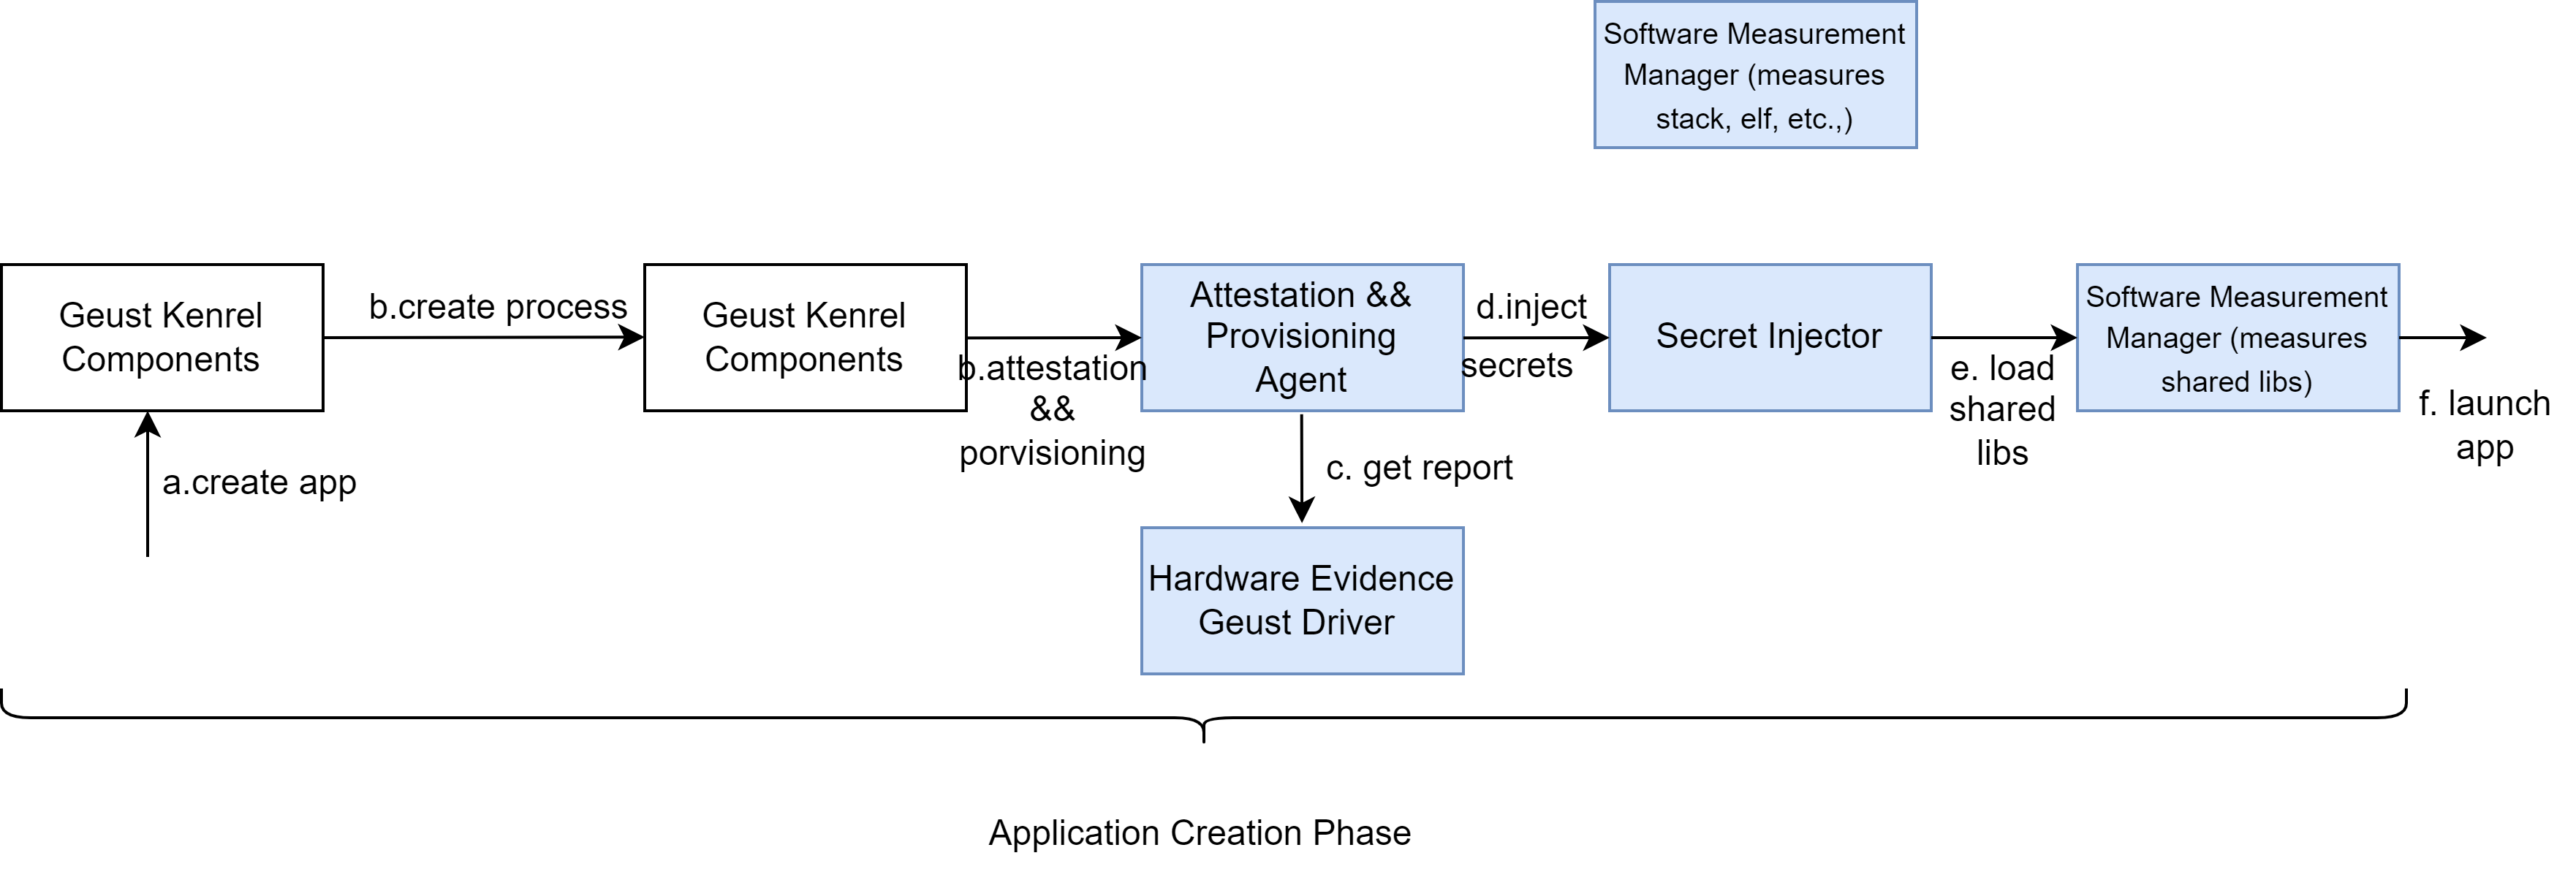
\includegraphics[width=0.8\textwidth]{images/micro_benchmark_app_life_cycle_bencmark_pattern.png}
    \caption[Benchmark Pattern - Latency Test for Application Startup]{Benchmark Pattern - Latency Test for Application Startup}
    \label{fig:micro_benchmark_app_life_cycle_bencmark_pattern}
\end{figure}


Regarding the benchmark methodology. A statically linked hello-world program in list 1 is used. To reduce the interference of environmental noise,the test framework runs the application 100 times. In addition, since the remote attestation and provisioning agent, the secret injector, 
the hardware evidence driver, and the software measurement manager shown in Figure  ~\ref{fig:micro_benchmark_app_life_cycle_bencmark_pattern}  (colored boxes) are located in the guest kernel, the test framework cannot directly measure the time spent by these components. Therefore, we use guest clock\_gettime(monotonic) to record the time and print the 
latency overhead of each component to the host using the qkernel logging system. The same approach applies to record the size of data measured by the software measurement manager. 


As expounded in Chapter 4, two factors may impact the application startup time in Cquark: the number of file type secrets and the size of the data measured by the software measurement manager. Hence, this section conducts following three tests. First, we establish a baseline by setting the 
number of file-type secrets to zero and running the hello world program. The test framework measures the program startup time, and records the latency overhead from the remote attestation and provisioning agent, the secret injector, the hardware evidence driver, and the software measurement manager。  
In Experiment 2, we increase the number of file type secrets in order to observe the change in program startup time, as well as the latency overhead from the remote proof and upgrade agent and the secret injector. In Experiment 3, we examine the growth in the latency overhead of the software 
measurement manager during program startup as the amount of measured data increased. To conduct the test, we utilize a variant of the hello-world program as shown in Listing II, incorporating a global initialization array to regulate the data segment size in the binary and thus modify the size 
of software manager measured data during program startup.

\subsubsection{Creating a Baseline}

This benchmark measures the hello world program's startup time, and the latency overhead caused by remote attestation and provisioning agent, the secret injector, the hardware evidence driver, and the software measurement manager. Note that here the number of file type secrets is 0.

\begin{figure}[H]
    \centering
    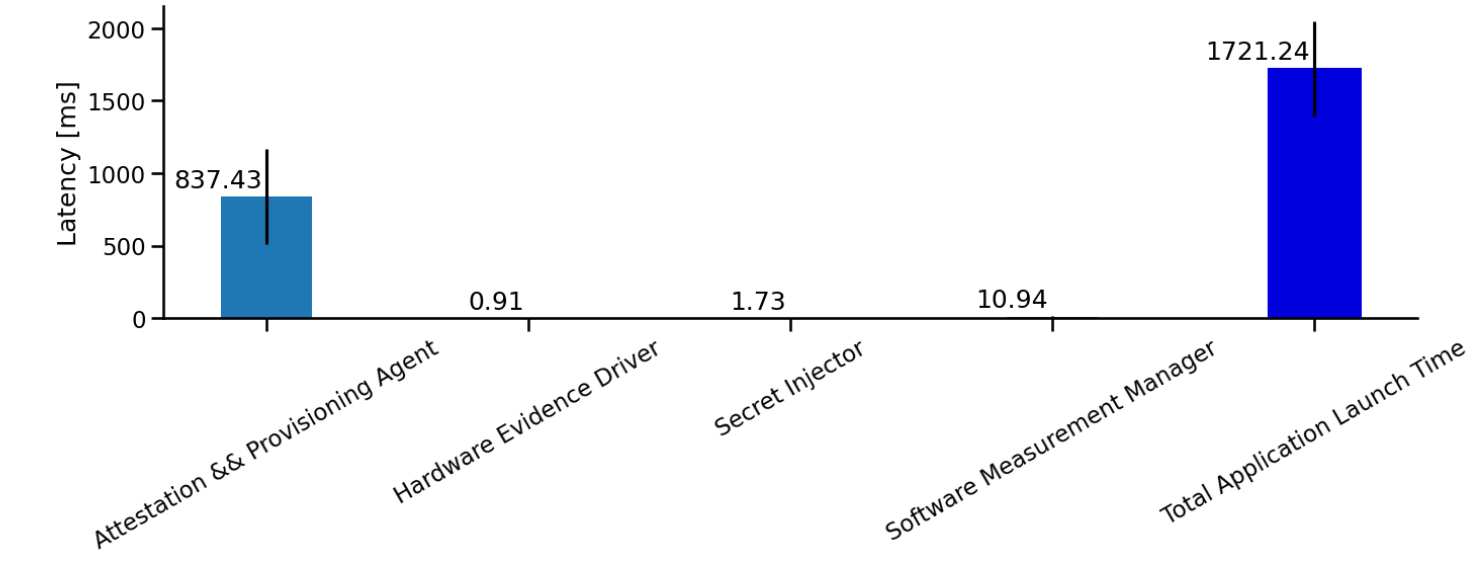
\includegraphics[width=0.8\textwidth]{images/application_start_microtest_baseline_time_overhead_each_cmp.PNG}
    \caption[Benchmark results: Latency Overhead introduce by new Componnents in Cquark]{Benchmark results: Latency Overhead introduce by new Componnents in Cquark}
    \label{fig:application_start_microtest_baseline_time_overhead_each_cmp}
\end{figure}

\begin{figure}[H]
    \centering
    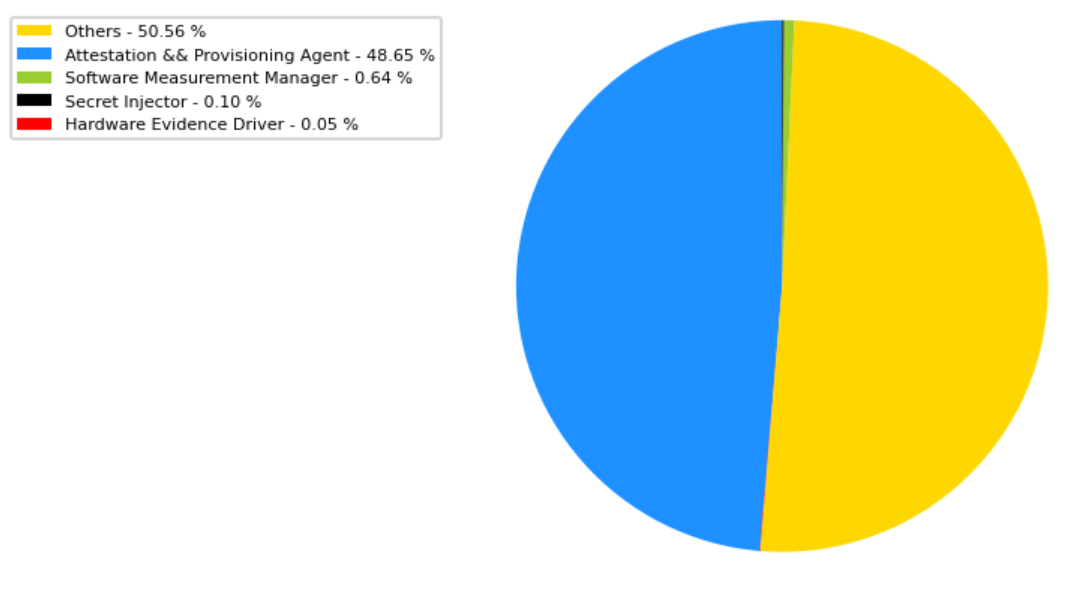
\includegraphics[width=0.8\textwidth]{images/application_start_microtest_baseline_time_distribution.PNG}
    \caption[Time  Distribution of the application startup ]{Distribution of the time consumed by different components in the application startup}
    \label{fig:application_start_microtest_baseline_time_distribution}
\end{figure}



The benchmark results in figure ~\ref{fig:application_start_microtest_baseline_time_overhead_each_cmp} and ~\ref{fig:application_start_microtest_baseline_time_distribution}  shows that the remote attestation and provisioning agent, the secret injector, the hardware evidence driver, and the software measurement manager doubled the program startup time. Notably, the remote attestation and provisioning agent contributed the most to the latency 
overhead, which is expected, given its necessity to establish a TLS connection with the relying party, complete the remote attestation process, and fetch the shield layer policy following the KBS attestation protocol. With regards to the secret injector, the hardware evidence object driver, 
which is primarily responsible for loading secrets into the application process and generating a simulated hardware report accordingly,  exhibited a delay overhead of 0.90 milliseconds and 1.73 milliseconds, respectively. However, this delay is negligible compared to the overhead caused 
by the remote attestation and provisioning agent (~837 milliseconds).  Furthermore, according to Table , based on the data presented in Table ~\ref{table: Measurement_For_Hello_world}, the software measurement manager is found to measure approximately 1.45 MiB of data during program startup, leading to an overhead of only about 
10 milliseconds.

\begin{table}[htbp]
    \centering
    \footnotesize
    \caption{Software measurement manager measured data during application startup\strut}
    \begin{tabularx}{1\textwidth}{@{} l L L L L L L@{}}
    \toprule
        Matrics    & ELF &  Shared Library   & Process Spec  & Stack   & Guest Kernel Args  & Total Measurement\\
    \midrule

        \vn{Measurement}     &  1.447 MiB    &   0 MiB  &   3819 Byte   & 305 Byte   &5865 Byte  & 1.457 MiB\\
    \bottomrule
    \end{tabularx}
    \label{table: Measurement_For_Hello_world}
\end{table}



\subsubsection{Determining Attestation \&\& Provisioning Agent and Secret Injector Overhead}
The baseline results confirm that the remote attestation and provisioning agent are significant source of latency overhead. To this end, this section aims to examine how the latency overhead of the remote attestation and provisioning agent, along with the secret injector, changes as the number 
of file-type secrets increases. Please see paragraph xx for additional information on the benchmark configuration.

\begin{figure}[H]
    \centering
    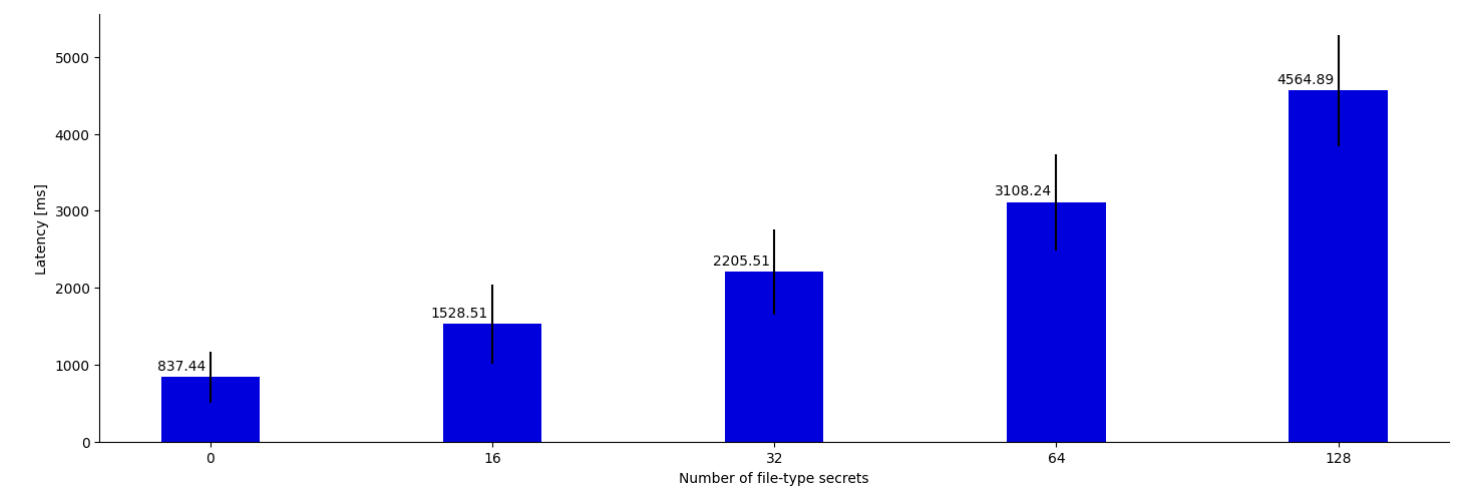
\includegraphics[width=0.8\textwidth]{images/overhead_attestation_agent_as_file_num_increasing.PNG}
    \caption[Benchmark result: Latency Overhead from Attestation \&\& Provisioning Agent as the number of file-based secrets increases]{Benchmark result: Latency Overhead from Attestation \&\& Provisioning Agent as the number of file-based secrets increases}
    \label{fig:overhead_attestation_agent_as_file_num_increasing}
\end{figure}

\begin{figure}[H]
    \centering
    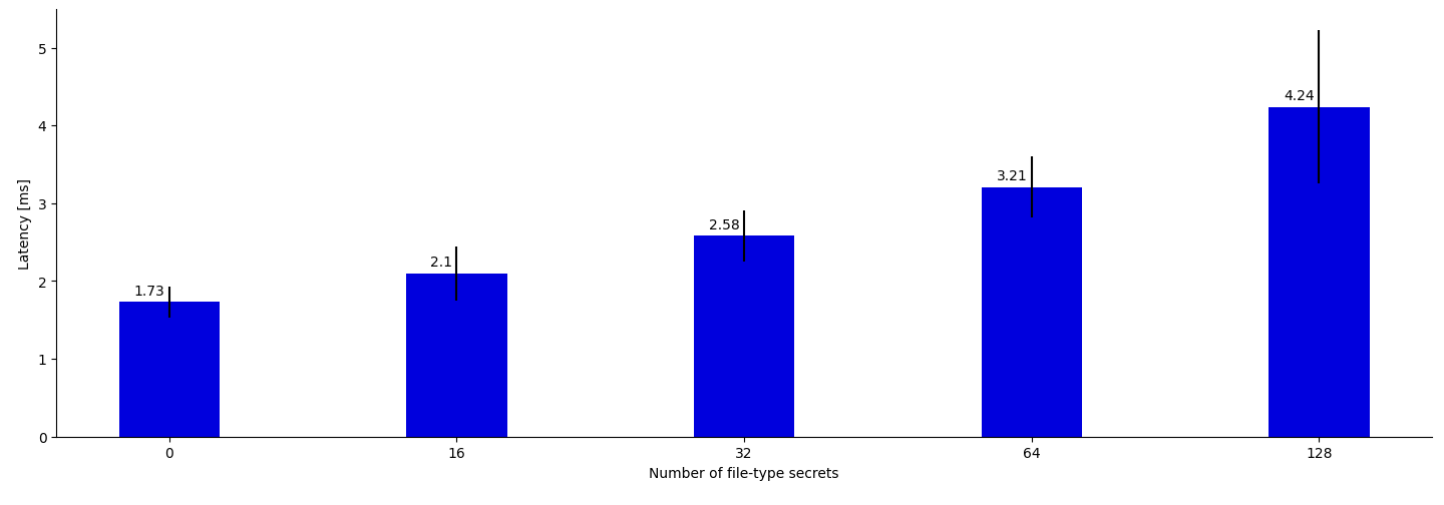
\includegraphics[width=0.8\textwidth]{images/overhead_secret_injector_as_file_num_increasing.PNG}
    \caption[Benchmark result: Latency Overhead from Secret Injector as the number of file-based secrets increases]{Benchmark result: Latency Overhead from Secret Injector as the number of file-based secrets increases}
    \label{fig:overhead_secret_injector_as_file_num_increasing}
\end{figure}


This paragraph discusses the benchmark results in Figure ~\ref{fig:overhead_attestation_agent_as_file_num_increasing} and Figure ~\ref{fig:overhead_secret_injector_as_file_num_increasing}, which reveal the evolution of the overhead introduced by the remote attestation and provisioning agent, and secret injector, as the number of file-type secrets grows. The results demonstrate that the increase in 
overhead from the remote attestation and provisioning agent, and secret injector, is proportional to the number of file-type secrets, as expected. As discussed in Chapter 5, constrained by the maximum TLS record size supported by the embedded\_tls library (16kb), the remote attestation and provisioning 
agent must perform one HTTP get + tls operation for each file-type secret. For the secret injector, it is evident that as the number of files increases, it needs more time to inject the files into the target location in the application process.  Additionally, a 
Figure ~\ref{fig:startup_time_change_as_file_type_secret_increasing} reveals that although the overhead from the secret injector increases as the number of file secrets grows, it is negligible compared to the overhead from remote attestation and provisioning agent. Moreover, when the number of file-type secrets reaches 128, 
the overhead associated with the remote attestation and provisioning agents becomes astounding, reaching 4500 ms, accounting for over 70\% of the total program startup time.

\begin{figure}[H]
    \centering
    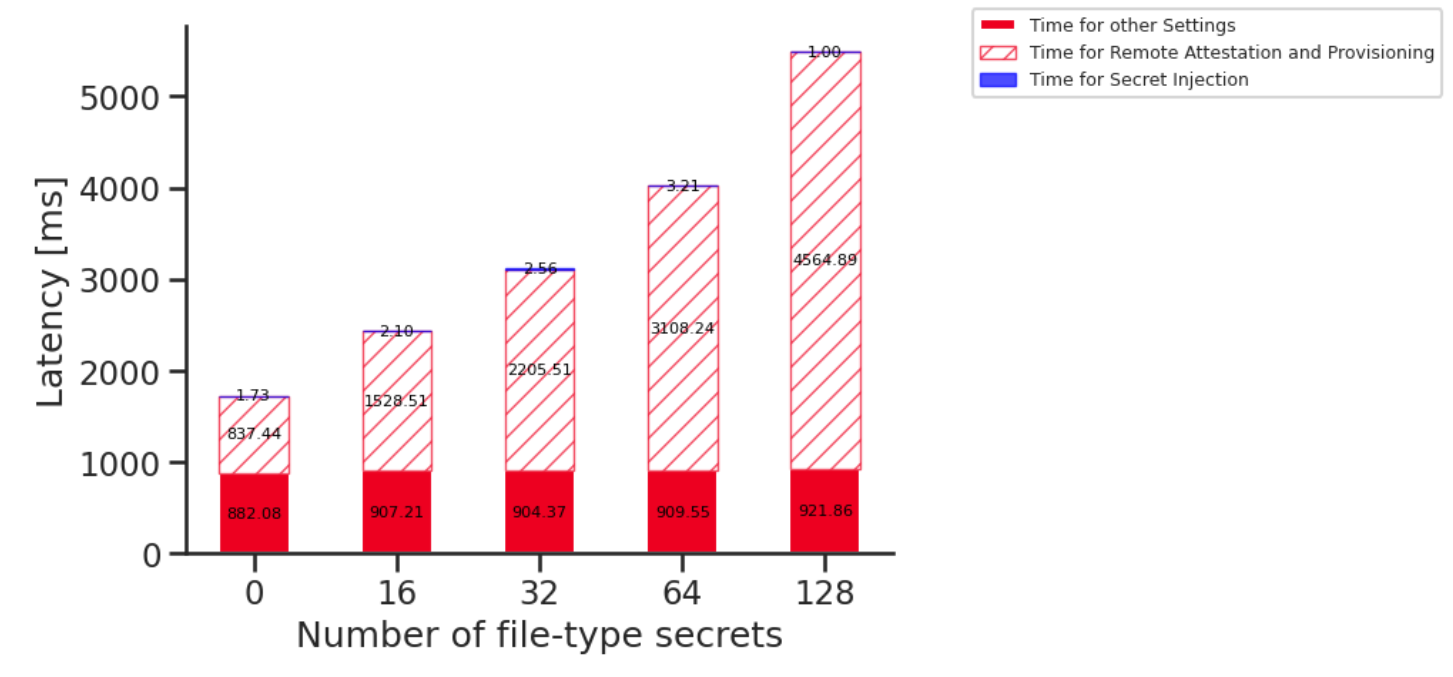
\includegraphics[width=0.8\textwidth]{images/startup_time_change_as_file_type_secret_increasing.PNG}
    \caption[Distribution of the time consumed by attestation \&\& provisioning agent, secret injector and others in the application startup]{Distribution of the time consumed by attestation \&\& provisioning agent, secret injector and others in the application startup}
    \label{fig:startup_time_change_as_file_type_secret_increasing}
\end{figure}



\subsubsection{Impact of measured Data Size}
This benchmark assesses the changes in the software measurer's latency overhead as the application binary size grows. Please refer to paragraph xx for the benchmark configuration.

\begin{figure}[H]
    \centering
    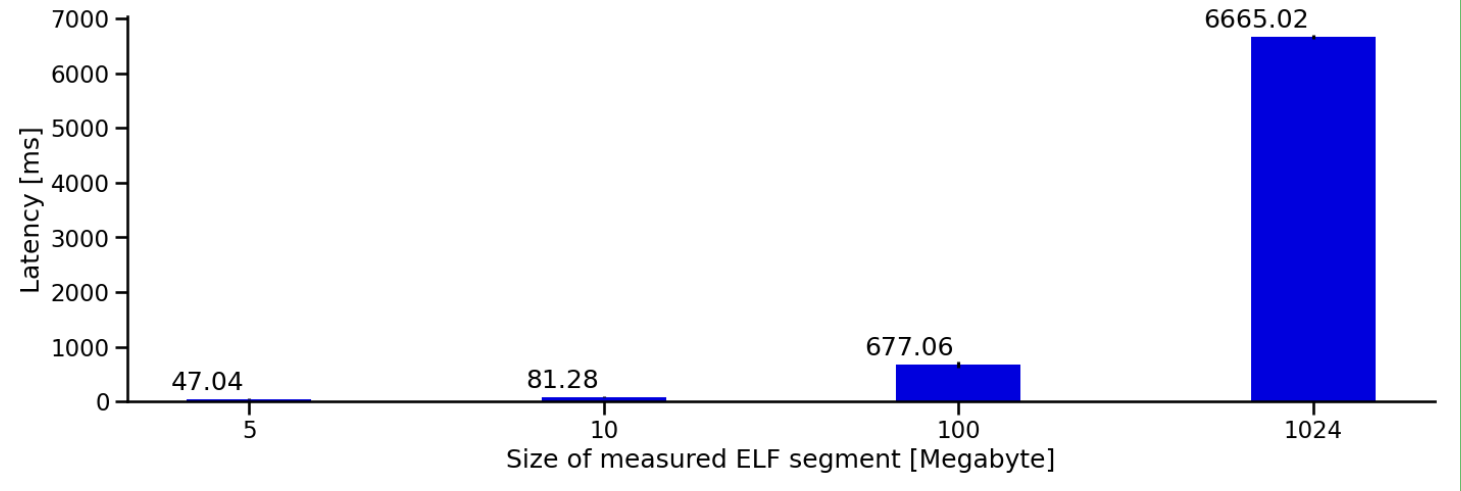
\includegraphics[width=0.8\textwidth]{images/overhead_software_measurement_manager_as_elf_size_increasing.PNG}
    \caption[Benchmark result: Latency Overhead from Software Measurement Manager as the measured Data Size increases]{Benchmark result: Latency Overhead from Software Measurement Manager as the measured Data Size increases}
    \label{fig:overhead_software_measurement_manager_as_elf_size_increasing}
\end{figure}

\begin{figure}[H]
    \centering
    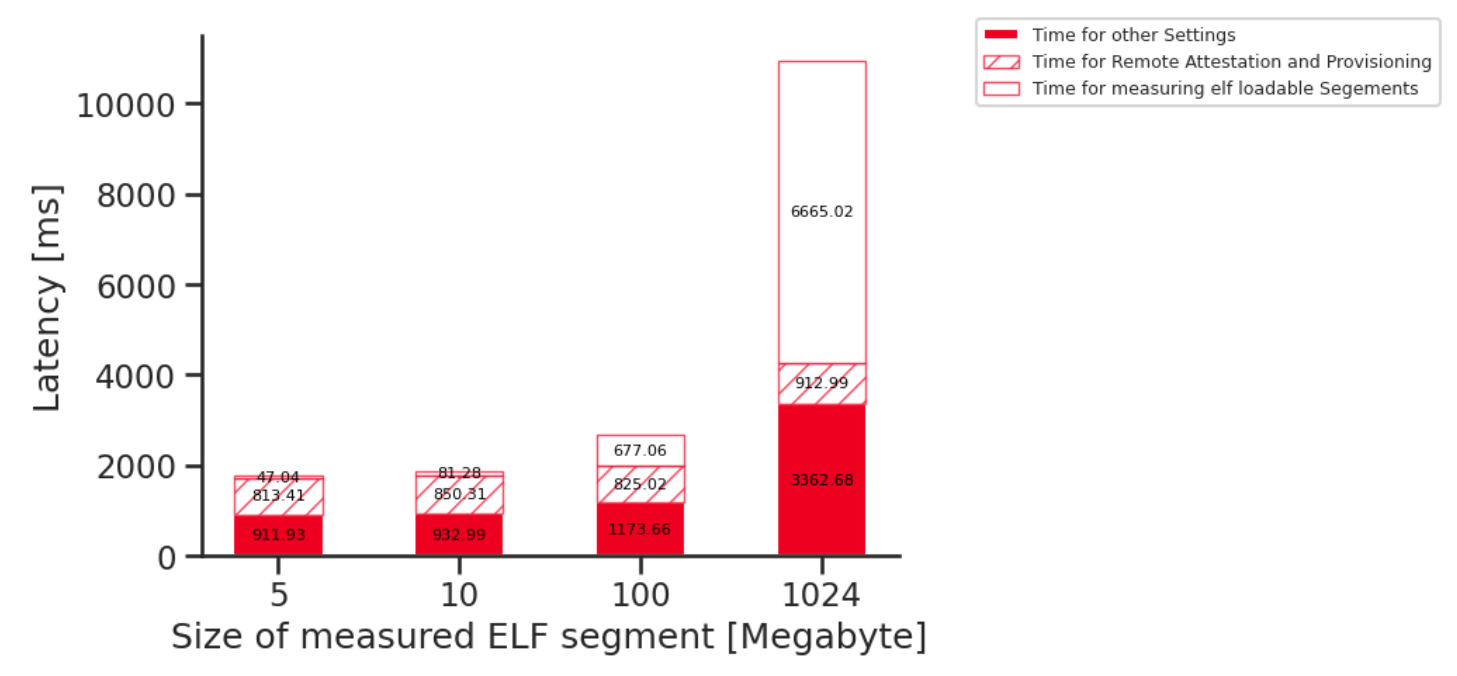
\includegraphics[width=0.8\textwidth]{images/startup_time_change_as_elf_size_increasing.PNG}
    \caption[Distribution of the time consumed by Attestation \&\& Provisioning Agent, Software Measurement Manager and others in the Application Startup]{Distribution of the time consumed by Attestation \&\& Provisioning Agent, Software Measurement Manager and others in the Application Startup}
    \label{fig:startup_time_change_as_elf_size_increasing}
\end{figure}



The benchmark results are in Figure ~\ref{fig:overhead_software_measurement_manager_as_elf_size_increasing}, which shows the latency overhead of the software measurer is proportional to the binary file size, i.e., the more data to be measured, the higher the overhead introduced by the software measurer. Furthermore, it is worth mentioning that when measured 
data less than or equal to 100 MiB, the latency overhead of the software measurer is lower than the overhead introduced by the remote attestation and provisioning agent. (Figure ~\ref{fig:startup_time_change_as_elf_size_increasing}).



\subsection{Macro-Benchmark– Application Life Cycle Performance Benchmark}

To evaluate the performance of Cquark in a real-world scenario, we conducted the following macro benchmark. The test compares the startup time, exit time, and runtime throughput of real-world applications in Cquark and vanilla quark using Nginx and Redis. It should be noted that program startup time 
is measured from the start of the Qkernel to the completion of the dynamic linker (ld.so) loading the application's shared libraries, while the program exit time refers to the time from the time the exit system call is called until qkernel stops running, as shown in Figure 1. Regarding the application 
runtime throughput, we use the Apache HTTP server benchmarking tool (AB) and Redis-benchmark to generate workloads for Nginx and Redis, respectively


Regarding the benchmark methodology and setup, our testing framework was extended to launch the target application repeatedly, record its startup and exit times, and results from AB and Redis-benchmark. Specifically, the test framework launches the target application 100 times, with the remote 
attestation and provisioning agent only fetching the shield policy from the relying party. For workload generator’s configuration, Redis benchmark and AB are set to issue 1,000,000 requests using 50 concurrent clients to Redis and Nginx, respectively. In addition, the size of the file requested 
by ab to Nginx is 181 bytes. In addition, the size of the file requested by ab to Nginx is 181 bytes.

\begin{figure}[H]
    \centering
    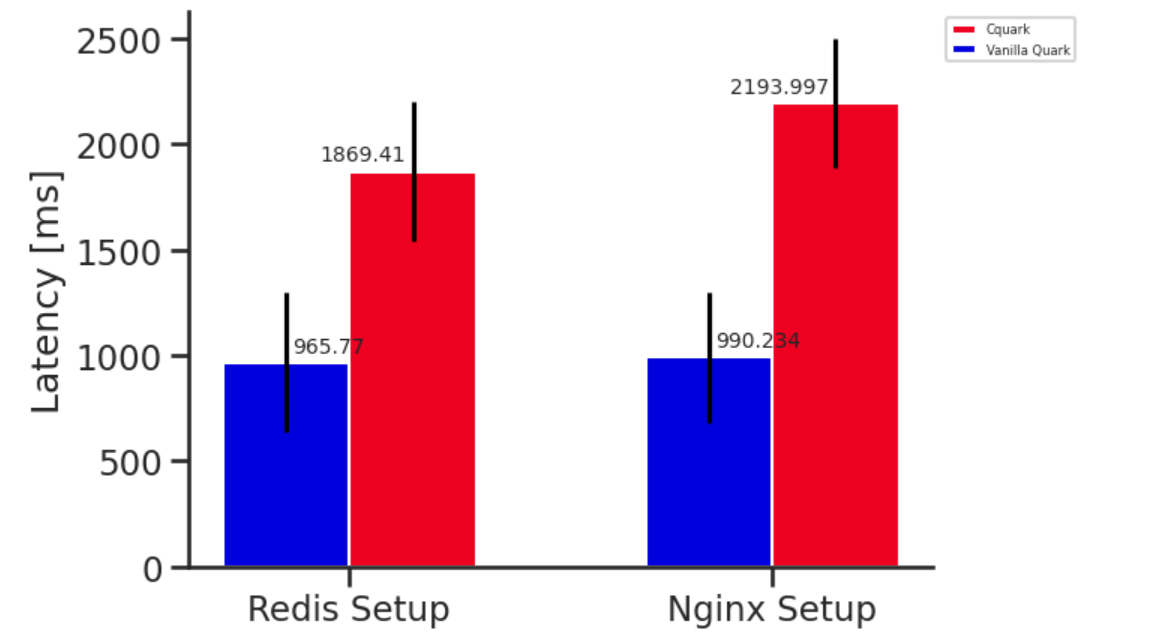
\includegraphics[width=0.8\textwidth]{images/reds_nginx_startup_comp.PNG}
    \caption[Redis \&\& Nginx Startup Time in Cquark vs vanilla Quark]{Redis \&\& Nginx Startup Time in Cquark vs vanilla Quark}
    \label{fig:reds_nginx_startup_comp}
\end{figure}

The results presented in Figure ~\ref{fig:reds_nginx_startup_comp} indicate that Cquark takes about twice as long as vanilla quark to complete the application setup. This result is reasonable, given that Qkernel in Cquark must perform additional operations like remote attestation, secret provisioning, and host loaded data 
measurement, which prolongs the startup time of an application. When comparing the startup time of Nginx and Redis in the Cquark(~\ref{fig:reds_nginx_startup_comp}), we observed that Nginx takes approximately  324 ms longer than Redis to start. Since both applications only fetch the shield policy 
during startup, the latency overhead from the remote attestation and provisioning agent should be identical for both. Therefore, we deduce that the longer Nginx startup time is due to the software measurement manager measuring more data, resulting in an increased startup time.

\begin{figure}[H]
    \centering
    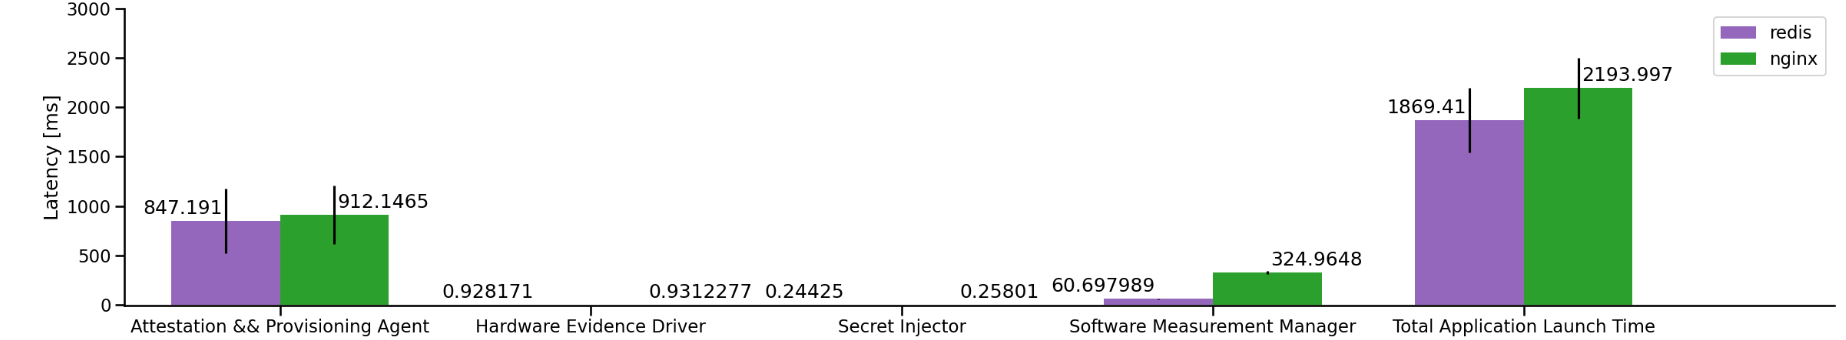
\includegraphics[width=0.8\textwidth]{images/time_disribution_startup_redis_nginx.PNG}
    \caption[Redis \&\& Nginx  Startup Time in Cquark vs vanilla Quark]{Redis \&\& Nginx  Startup Time in Cquark vs vanilla Quark}
    \label{fig:time_disribution_startup_redis_nginx}
\end{figure}

\begin{table}[htbp]
    \centering
    \footnotesize

    \begin{tabularx}{1\textwidth}{@{} l L L L L L L@{}}
    \toprule
        Matrics    & ELF &  Shared Library   & Process Spec  & Stack   & Guest Kernel Args  & Total Measurement\\
    \midrule

        \vn{Measurement for Redis}     &  3.64 MiB   &   12.61 MiB  &   3476 Byte   & 310 Byte   &5865 Byte  & 16.26 MiB\\
        \vn{Measurement for Nginx}     &  5.5 MiB    &   61.64 MiB  &   3352 Byte  & 2169 Byte  &5865 Byte  & 67.15 MiB\\
    \bottomrule
    \end{tabularx}
    \caption{Software Measurement Manager measured Data during Application Startup\strut}
    \label{table: Measurement_For_Nginx_Redis}
\end{table}


To validate our hypothesis, we measured the overhead induced by the remote attestation and provisioning agent, the secret injector, the hardware evidence driver, and the software measurement manager, as well as the size of the data measured by the software measurer during the application 
startup in Cquark. The relevant details can be found in Figure  ~\ref{fig:time_disribution_startup_redis_nginx} and Table ~\ref{table:Measurement_For_Nginx_Redis}. Our findings show that the software measurer measured 16.25 MiB and 67.15 MiB of data for Redis and Nginx respectively, leading to a latency of 60.69 ms and 324 ms.   Additionally, even though both applications 
have the same setup for the remote attestation and provisioning agent, the difference in latency overhead from the remote attestation and provisioning agent due to possible network transmission jitter was approximately 65 ms. Moreover, the latency generated from the hardware evidence driver and 
secret injection was less than 1 ms in both cases, which was insignificant compared to the software measurer and remote attestation and provisioning agent's overhead. To summarize, Nginx's startup time is longer compared to Redis due to two key reasons - network jitter and Nginx requires the 
software measurement manager to process more data during setup.

\begin{figure}[H]
    \centering
    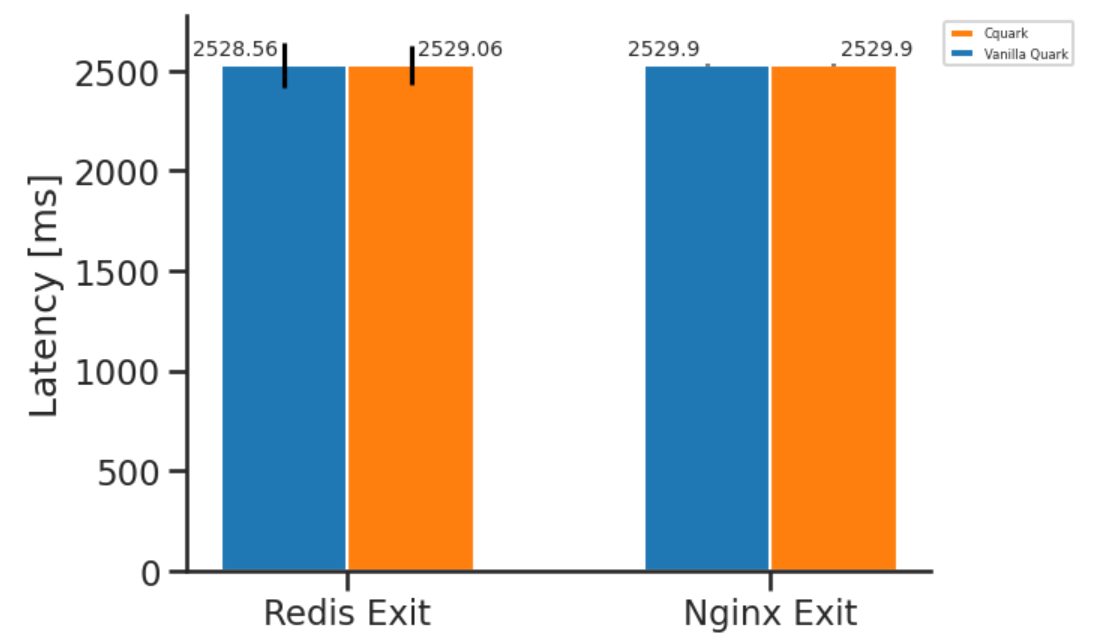
\includegraphics[width=0.8\textwidth]{images/reds_nginx_exit_comp.PNG}
    \caption[Redis \&\& Nginx Exit Time in Cquark vs vanilla Quark]{Redis \&\& Nginx Exit Time in Cquark vs vanilla Quark}
    \label{fig:reds_nginx_exit_comp}
\end{figure}


With respect to the application (sandbox) exit, Figure ~\ref{fig:reds_nginx_exit_comp}  shows that Cquarkcan achieves the same performance as vanilla Quark. Specifically, in both Cquark and vanilla quark, the exit time of Redis and Nginx is around 2529 ms.

\begin{figure}[H]
    \centering
    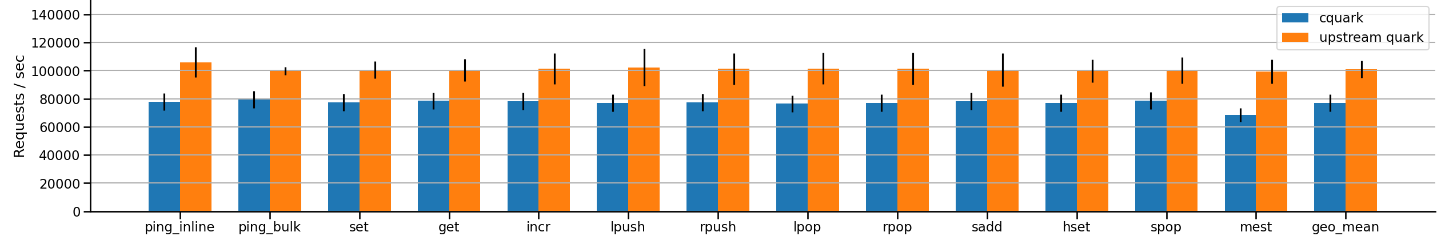
\includegraphics[width=1\textwidth]{images/redis_throughput.PNG}
    \caption[Redis Throughout Test]{Redis Throughout Test Result}
    \label{fig:redis_throughput}
\end{figure}


\begin{figure}[H]
    \centering
    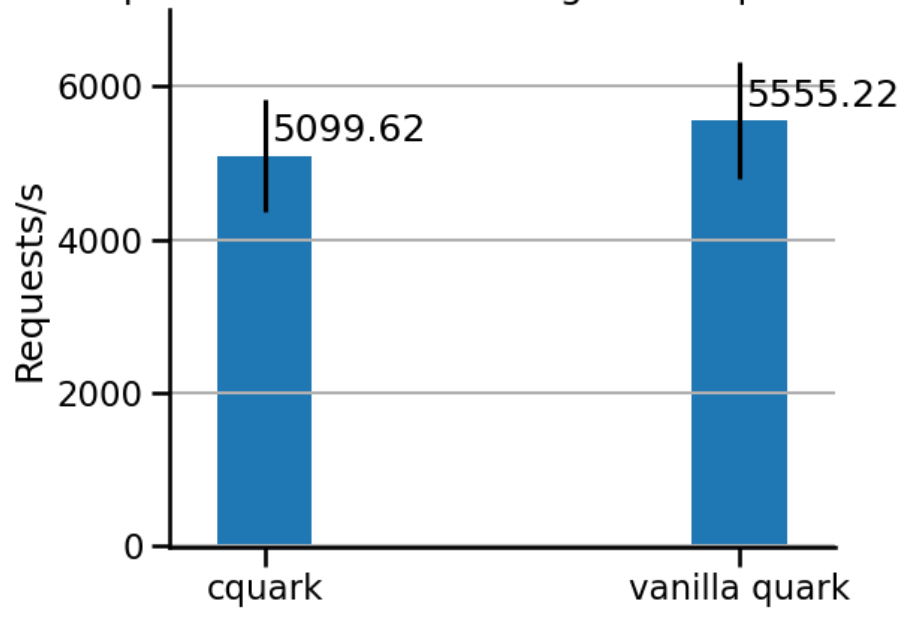
\includegraphics[width=1\textwidth]{images/nginx_throughput.PNG}
    \caption[Nginx Throughout Test]{Nginx Throughout Test Result}
    \label{fig:nginx_throughput}
\end{figure}


The throughput test results for Redis and Nginx can be found in Figures ~\ref{fig:redis_throughput} and  ~\ref{fig:nginx_throughput}, respectively. Our analysis shows that execution of Redis and Nginx in Cquark led to a performance degradation of approximately 22\% and 10\%, respectively. The primary reason for this effect is the interception of 
the guest system calls.



\subsection{Trust Computing Base}



In VM-based Trusted Execution Environments (TEE), the Trusted Computing Base (TCB) comprises the necessary hardware, firmware, and software modules, like the guest operating system, that ensure the required security guarantee while handling confidential data. The smaller the TCB, the lower the 
risk of a TEE being compromised by a vulnerability. Therefore, in this section, we evaluate the TCB overhead introduced by our implementation and compares the TCB size between CQuark and Confidential Container. To assess CQuark-incurred TCB overhead, we compare the lines of code and the size of 
the guest kernel binary in CQuark and vanilla Quark as both use a application kernel as the guest kernel and the shield layer is part of  the guest kernel binary.  For the TCB size comparison between CQuark and the Confidential Container, we use the binary size of the Guest assets as a reference.  
To ensure fairness, we employ the strip utility to remove unused symbols in binaries.

\begin{table}[htbp]
    \centering
\begin{tabular}{lrrrcrrr}\toprule
    \hline
    \multicolumn{3}{c}{Vanilla Quark}&&\multicolumn{3}{c}{Confidential Quark}\\
    \cline{1-3}\cline{5-7}
    $Component$ & $LoC$ & $Size$$^{3}$ && $Component$ & $LoC$ & $Size$$^{3}$\\
  \midrule
     Qkernel &32487 & -&& Qkernel&32487&-\\
     Qlib &85128  & -&&Qlib&  86609 &-\\
     Shield  & 0 & - && Shield&2805&-\\
  
     \midrule
      Total  & 117615& 3.1MiB&& & 121901 &  4.6 MiB\\
      \bottomrule
  \end{tabular}

  \caption{Comparison of the LoC and compiled size of vanilla quark and confidential quark\strut}
  \label{table:tcb_size_quark_vs_cquark}
\end{table}

Table ~\ref{table:tcb_size_quark_vs_cquark} provides a summary of the TCB overhead required to achieve confidentiality in CQuark. The Vanilla Quark version v2.0 has a guest kernel with 11,7615 lines of code and generates a 3.10 MB static linked binary. In CQuark, our implementation adds 4286 LoC to the guest binary, bringing the total to 12,1901
LoC and 4.6 MB of compiled static linked binary. Overall, our implementation makes the qkernel binary 1.48 times larger compared to Vanilla Quark.


\begin{table}[htbp]
    \centering
\begin{tabular}{lrrcrr}\toprule
    \hline
    \multicolumn{2}{c}{Confidential Container}&&\multicolumn{2}{c}{Confidential Quark}\\
    \cline{1-2}\cline{4-5}
    $Component$  & $Size$$^{3}$ && $Component$  & $Size$$^{3}$\\
  \midrule
     Guest Kernel & 22.65MiB&& Guest kernel &4.6 MiB\\
     OVMF   & 4 MiB && &   &\\
     Kata agent  & 47.16 MiB  && &&\\
  
     \midrule
        & 73.81 MB&& &   4.6 MiB\\
      \bottomrule
  \end{tabular}

  \caption{TCB size comparison between confidential container vs confidential quark in terms of compiled size of guest assets \strut}
  \label{table:tcb_size_quark_vs_kata}
\end{table}

Table ~\ref{table:tcb_size_quark_vs_kata} shows the outcomes of comparing the TCB size in the Confidential Container (Kata) and CQuark. Unlike CQuark, which uses the application kernel as the guest kernel, Confidential Container deploys the qemu-linux base virtual machine. Therefore, the guest assets in the Confidential Container 
context include the Kata agent, OVMF, and Linux Guest kernel. In the Confidential Container version v0.4, the compiled static binary sizes of Kata agent, OVMF, and Guest kernel are 22.65 Mb, 4.0 MB, and 47.16 MB, respectively. This totals a TCB size of 73.81 MB, which is about 16 times greater than that 
of CQuark.

It is noteworthy that there is potential to further optimize the size of Quark's Trusted Computing Base (TCB).  In Quarkv version 2.0, qlib contributes some redundant code to qkernel. To facilitate code development, the qlib code is shared between qvisor and qkernel. However, our founding shows 
some code in qlib is only used by functions in qvisor, thus increasing the size of the qkernel’s binary. 




% \begin{table}[htp]
%     \caption{Software measurement manager measured data during application startup}
%     \begin{tabularx}{\textwidth}{*{2}{p{0.5\textwidth}}}\toprule
%                                  & ELF &  Shared Library   & Process Spec  & Stack   & Guest Kernel Args  & Total Measurement \\ \midrul
%     Measurement For Hello world  &  1.4468 MiB    &   0 MiB  &   3819 Byte   & 305 Byte   &5865 Byte  & 1.457 MiB \\\addlinespace
%     \bottomrule
%     \end{tabular}
%     \label{table: Measurement_For_Hello_world}
% \end{table}


% \begin{table}[!ht]
%     \sffamily
%     \caption{Terminologies in SQL \& corresponding in MongoDB}
%     \label{tab:my_label}
%     \centering
%     \begin{tabularx}{\textwidth}{*{2}{p{0.5\textwidth}}}
%     \toprule
%                                  & ELF &  Shared Library   & Process Spec  & Stack   & Guest Kernel Args  & Total Measurement \\ \midrule
%     Measurement For Hello world  &  1.4468 MiB    &   0 MiB  &   3819 Byte   & 305 Byte   &5865 Byte  & 1.457 MiB \\\addlinespace
%     \dots & \dots \\
%     \bottomrule
%     \end{tabularx}
%     \end{table}




\cleardoublepage

%%% Local Variables:
%%% TeX-master: "diplom"
%%% End:
